\documentclass[twoside]{book}

% Packages required by doxygen
\usepackage{fixltx2e}
\usepackage{calc}
\usepackage{doxygen}
\usepackage[export]{adjustbox} % also loads graphicx
\usepackage{graphicx}
\usepackage[utf8]{inputenc}
\usepackage{makeidx}
\usepackage{multicol}
\usepackage{multirow}
\PassOptionsToPackage{warn}{textcomp}
\usepackage{textcomp}
\usepackage[nointegrals]{wasysym}
\usepackage[table]{xcolor}

% Font selection
\usepackage[T1]{fontenc}
\usepackage[scaled=.90]{helvet}
\usepackage{courier}
\usepackage{amssymb}
\usepackage{sectsty}
\renewcommand{\familydefault}{\sfdefault}
\allsectionsfont{%
  \fontseries{bc}\selectfont%
  \color{darkgray}%
}
\renewcommand{\DoxyLabelFont}{%
  \fontseries{bc}\selectfont%
  \color{darkgray}%
}
\newcommand{\+}{\discretionary{\mbox{\scriptsize$\hookleftarrow$}}{}{}}

% Page & text layout
\usepackage{geometry}
\geometry{%
  a4paper,%
  top=2.5cm,%
  bottom=2.5cm,%
  left=2.5cm,%
  right=2.5cm%
}
\tolerance=750
\hfuzz=15pt
\hbadness=750
\setlength{\emergencystretch}{15pt}
\setlength{\parindent}{0cm}
\setlength{\parskip}{3ex plus 2ex minus 2ex}
\makeatletter
\renewcommand{\paragraph}{%
  \@startsection{paragraph}{4}{0ex}{-1.0ex}{1.0ex}{%
    \normalfont\normalsize\bfseries\SS@parafont%
  }%
}
\renewcommand{\subparagraph}{%
  \@startsection{subparagraph}{5}{0ex}{-1.0ex}{1.0ex}{%
    \normalfont\normalsize\bfseries\SS@subparafont%
  }%
}
\makeatother

% Headers & footers
\usepackage{fancyhdr}
\pagestyle{fancyplain}
\fancyhead[LE]{\fancyplain{}{\bfseries\thepage}}
\fancyhead[CE]{\fancyplain{}{}}
\fancyhead[RE]{\fancyplain{}{\bfseries\leftmark}}
\fancyhead[LO]{\fancyplain{}{\bfseries\rightmark}}
\fancyhead[CO]{\fancyplain{}{}}
\fancyhead[RO]{\fancyplain{}{\bfseries\thepage}}
\fancyfoot[LE]{\fancyplain{}{}}
\fancyfoot[CE]{\fancyplain{}{}}
\fancyfoot[RE]{\fancyplain{}{\bfseries\scriptsize Generated by Doxygen }}
\fancyfoot[LO]{\fancyplain{}{\bfseries\scriptsize Generated by Doxygen }}
\fancyfoot[CO]{\fancyplain{}{}}
\fancyfoot[RO]{\fancyplain{}{}}
\renewcommand{\footrulewidth}{0.4pt}
\renewcommand{\chaptermark}[1]{%
  \markboth{#1}{}%
}
\renewcommand{\sectionmark}[1]{%
  \markright{\thesection\ #1}%
}

% Indices & bibliography
\usepackage{natbib}
\usepackage[titles]{tocloft}
\setcounter{tocdepth}{3}
\setcounter{secnumdepth}{5}
\makeindex

% Hyperlinks (required, but should be loaded last)
\usepackage{ifpdf}
\ifpdf
  \usepackage[pdftex,pagebackref=true]{hyperref}
\else
  \usepackage[ps2pdf,pagebackref=true]{hyperref}
\fi
\hypersetup{%
  colorlinks=true,%
  linkcolor=blue,%
  citecolor=blue,%
  unicode%
}

% Custom commands
\newcommand{\clearemptydoublepage}{%
  \newpage{\pagestyle{empty}\cleardoublepage}%
}

\usepackage{caption}
\captionsetup{labelsep=space,justification=centering,font={bf},singlelinecheck=off,skip=4pt,position=top}

%===== C O N T E N T S =====

\begin{document}

% Titlepage & ToC
\hypersetup{pageanchor=false,
             bookmarksnumbered=true,
             pdfencoding=unicode
            }
\pagenumbering{alph}
\begin{titlepage}
\vspace*{7cm}
\begin{center}%
{\Large My Project }\\
\vspace*{1cm}
{\large Generated by Doxygen 1.8.13}\\
\end{center}
\end{titlepage}
\clearemptydoublepage
\pagenumbering{roman}
\tableofcontents
\clearemptydoublepage
\pagenumbering{arabic}
\hypersetup{pageanchor=true}

%--- Begin generated contents ---
\chapter{Hierarchical Index}
\section{Class Hierarchy}
This inheritance list is sorted roughly, but not completely, alphabetically\+:\begin{DoxyCompactList}
\item \contentsline{section}{util\+:\+:Date}{\pageref{classutil_1_1Date}}{}
\item logic\+\_\+error\begin{DoxyCompactList}
\item \contentsline{section}{Contrat\+Exception}{\pageref{classContratException}}{}
\begin{DoxyCompactList}
\item \contentsline{section}{Assertion\+Exception}{\pageref{classAssertionException}}{}
\item \contentsline{section}{Invariant\+Exception}{\pageref{classInvariantException}}{}
\item \contentsline{section}{Postcondition\+Exception}{\pageref{classPostconditionException}}{}
\item \contentsline{section}{Precondition\+Exception}{\pageref{classPreconditionException}}{}
\end{DoxyCompactList}
\end{DoxyCompactList}
\item \contentsline{section}{saaq\+:\+:Proprietaire}{\pageref{classsaaq_1_1Proprietaire}}{}
\item \contentsline{section}{saaq\+:\+:Vehicule}{\pageref{classsaaq_1_1Vehicule}}{}
\begin{DoxyCompactList}
\item \contentsline{section}{saaq\+:\+:Camion}{\pageref{classsaaq_1_1Camion}}{}
\item \contentsline{section}{saaq\+:\+:Vehicule\+Promenade}{\pageref{classsaaq_1_1VehiculePromenade}}{}
\end{DoxyCompactList}
\end{DoxyCompactList}

\chapter{Class Index}
\section{Class List}
Here are the classes, structs, unions and interfaces with brief descriptions\+:\begin{DoxyCompactList}
\item\contentsline{section}{\hyperlink{classAssertionException}{Assertion\+Exception} \\*Classe pour la gestion des erreurs d\textquotesingle{}assertion }{\pageref{classAssertionException}}{}
\item\contentsline{section}{\hyperlink{classsaaq_1_1Camion}{saaq\+::\+Camion} \\*Classe \hyperlink{classsaaq_1_1Camion}{Camion} qui contient les informations sur un \hyperlink{classsaaq_1_1Camion}{Camion} Contient la plaque d\textquotesingle{}immatriculation, la date d\textquotesingle{}enregistrement, le poid, le nombre d\textquotesingle{}essieu et le N\+IV du camion. Des méthode qui permettent de nous donner chaques valeurs. Une méthode qui permet d\textquotesingle{}assigner une nouvelle plaque de camion. Une méthode qui permet d\textquotesingle{}afficher le tout dans un format console }{\pageref{classsaaq_1_1Camion}}{}
\item\contentsline{section}{\hyperlink{classContratException}{Contrat\+Exception} \\*Classe de base des exceptions de contrat }{\pageref{classContratException}}{}
\item\contentsline{section}{\hyperlink{classutil_1_1Date}{util\+::\+Date} \\*Cette classe sert au maintien et à la manipulation des dates }{\pageref{classutil_1_1Date}}{}
\item\contentsline{section}{\hyperlink{classInvariantException}{Invariant\+Exception} \\*Classe pour la gestion des erreurs d\textquotesingle{}invariant }{\pageref{classInvariantException}}{}
\item\contentsline{section}{\hyperlink{classPostconditionException}{Postcondition\+Exception} \\*Classe pour la gestion des erreurs de postcondition }{\pageref{classPostconditionException}}{}
\item\contentsline{section}{\hyperlink{classPreconditionException}{Precondition\+Exception} \\*Classe pour la gestion des erreurs de précondition }{\pageref{classPreconditionException}}{}
\item\contentsline{section}{\hyperlink{classsaaq_1_1Proprietaire}{saaq\+::\+Proprietaire} \\*Classe \hyperlink{classsaaq_1_1Proprietaire}{Proprietaire} qui contient les Camions et \hyperlink{classsaaq_1_1Vehicule}{Vehicule} de promenade -\/\+Accesseurs pour tous ses attributs -\/\+Assigner une nouvelle plaque automobile -\/\+Une methode qui retourne le tout de facon formate }{\pageref{classsaaq_1_1Proprietaire}}{}
\item\contentsline{section}{\hyperlink{classsaaq_1_1Vehicule}{saaq\+::\+Vehicule} \\*Classe vehicule qui contient les informations d\textquotesingle{}une plaque automobile. Contient la plaque d\textquotesingle{}immatriculation, la date d\textquotesingle{}enregistrement et le N\+IV du vehicule. Des méthode qui permettent de nous donner chaques valeurs. Une méthode qui permet d\textquotesingle{}assigner une nouvelle plaque de vehicule. Une méthode qui permet d\textquotesingle{}afficher le tout dans un format console }{\pageref{classsaaq_1_1Vehicule}}{}
\item\contentsline{section}{\hyperlink{classsaaq_1_1VehiculePromenade}{saaq\+::\+Vehicule\+Promenade} \\*Classe \hyperlink{classsaaq_1_1VehiculePromenade}{Vehicule\+Promenade} qui contient les informations sur un \hyperlink{classsaaq_1_1Vehicule}{Vehicule} de Promenade Contient la plaque d\textquotesingle{}immatriculation, la date d\textquotesingle{}enregistrement, le nombre de place et le N\+IV du vehicule. Des méthode qui permettent de nous donner chaques valeurs. Une méthode qui permet d\textquotesingle{}assigner une nouvelle plaque de \hyperlink{classsaaq_1_1Vehicule}{Vehicule} de Promenade. Une méthode qui permet d\textquotesingle{}afficher le tout dans un format console }{\pageref{classsaaq_1_1VehiculePromenade}}{}
\end{DoxyCompactList}

\chapter{File Index}
\section{File List}
Here is a list of all documented files with brief descriptions\+:\begin{DoxyCompactList}
\item\contentsline{section}{\hyperlink{Camion_8cpp}{Camion.\+cpp} \\*Fichier d\textquotesingle{}implémentation de la classe Camion }{\pageref{Camion_8cpp}}{}
\item\contentsline{section}{\hyperlink{Camion_8h}{Camion.\+h} \\*Fichier déclaration de la classe Camion }{\pageref{Camion_8h}}{}
\item\contentsline{section}{\hyperlink{ContratException_8cpp}{Contrat\+Exception.\+cpp} \\*Implantation de la classe \hyperlink{classContratException}{Contrat\+Exception} et de ses héritiers }{\pageref{ContratException_8cpp}}{}
\item\contentsline{section}{\hyperlink{ContratException_8h}{Contrat\+Exception.\+h} \\*Fichier contenant la déclaration de la classe \hyperlink{classContratException}{Contrat\+Exception} et de ses héritiers }{\pageref{ContratException_8h}}{}
\item\contentsline{section}{\hyperlink{Date_8cpp}{Date.\+cpp} \\*Implantation de la classe Date }{\pageref{Date_8cpp}}{}
\item\contentsline{section}{\hyperlink{Date_8h}{Date.\+h} \\*Fichier qui contient l\textquotesingle{}interface de la classe Date qui sert au maintien et à la manipulation des dates }{\pageref{Date_8h}}{}
\item\contentsline{section}{\hyperlink{Proprietaire_8cpp}{Proprietaire.\+cpp} \\*Fichier d\textquotesingle{}implémentation de la classe Proprietaire }{\pageref{Proprietaire_8cpp}}{}
\item\contentsline{section}{\hyperlink{Proprietaire_8h}{Proprietaire.\+h} \\*Fichier declaration de la classe Proprietaire }{\pageref{Proprietaire_8h}}{}
\item\contentsline{section}{\hyperlink{validationFormat_8cpp}{validation\+Format.\+cpp} \\*Fichier permettant de valider une plaque automobile et un N\+IV }{\pageref{validationFormat_8cpp}}{}
\item\contentsline{section}{\hyperlink{validationFormat_8h}{validation\+Format.\+h} \\*Fichier permettant de valider une plaque automobile et un N\+IV }{\pageref{validationFormat_8h}}{}
\item\contentsline{section}{\hyperlink{Vehicule_8cpp}{Vehicule.\+cpp} \\*Fichier d\textquotesingle{}implémentation de la classe Vehicule }{\pageref{Vehicule_8cpp}}{}
\item\contentsline{section}{\hyperlink{Vehicule_8h}{Vehicule.\+h} \\*Fichier déclaration de la classe Vehicule }{\pageref{Vehicule_8h}}{}
\item\contentsline{section}{\hyperlink{VehiculePromenade_8cpp}{Vehicule\+Promenade.\+cpp} \\*Fichier d\textquotesingle{}implementation de la classe Vehicule\+Promenade }{\pageref{VehiculePromenade_8cpp}}{}
\item\contentsline{section}{\hyperlink{VehiculePromenade_8h}{Vehicule\+Promenade.\+h} \\*Fichier déclaration de la classe Vehicule\+Promenade }{\pageref{VehiculePromenade_8h}}{}
\end{DoxyCompactList}

\chapter{Class Documentation}
\hypertarget{classAssertionException}{}\section{Assertion\+Exception Class Reference}
\label{classAssertionException}\index{Assertion\+Exception@{Assertion\+Exception}}


Classe pour la gestion des erreurs d\textquotesingle{}assertion.  




{\ttfamily \#include $<$Contrat\+Exception.\+h$>$}



Inheritance diagram for Assertion\+Exception\+:\nopagebreak
\begin{figure}[H]
\begin{center}
\leavevmode
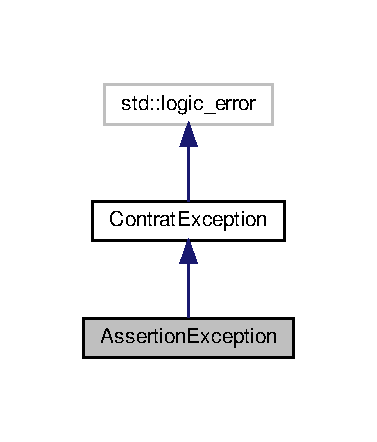
\includegraphics[width=181pt]{classAssertionException__inherit__graph}
\end{center}
\end{figure}


Collaboration diagram for Assertion\+Exception\+:\nopagebreak
\begin{figure}[H]
\begin{center}
\leavevmode
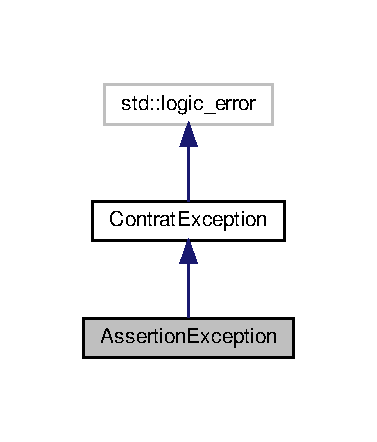
\includegraphics[width=181pt]{classAssertionException__coll__graph}
\end{center}
\end{figure}
\subsection*{Public Member Functions}
\begin{DoxyCompactItemize}
\item 
\hyperlink{classAssertionException_a93268f249b033bf4596901e50874fde6}{Assertion\+Exception} (std\+::string, unsigned int, std\+::string)
\begin{DoxyCompactList}\small\item\em Constructeur de la classe \hyperlink{classAssertionException}{Assertion\+Exception} ~\newline
 Le constructeur public \hyperlink{classAssertionException}{Assertion\+Exception}(...)initialise sa classe de base \hyperlink{classContratException}{Contrat\+Exception}. On n\textquotesingle{}a pas d\textquotesingle{}attribut local. Cette classe est intéressante pour son T\+Y\+PE lors du traitement des exceptions. \end{DoxyCompactList}\end{DoxyCompactItemize}


\subsection{Detailed Description}
Classe pour la gestion des erreurs d\textquotesingle{}assertion. 

\subsection{Constructor \& Destructor Documentation}
\mbox{\Hypertarget{classAssertionException_a93268f249b033bf4596901e50874fde6}\label{classAssertionException_a93268f249b033bf4596901e50874fde6}} 
\index{Assertion\+Exception@{Assertion\+Exception}!Assertion\+Exception@{Assertion\+Exception}}
\index{Assertion\+Exception@{Assertion\+Exception}!Assertion\+Exception@{Assertion\+Exception}}
\subsubsection{\texorpdfstring{Assertion\+Exception()}{AssertionException()}}
{\footnotesize\ttfamily Assertion\+Exception\+::\+Assertion\+Exception (\begin{DoxyParamCaption}\item[{std\+::string}]{p\+\_\+fichP,  }\item[{unsigned int}]{p\+\_\+prm\+Ligne,  }\item[{std\+::string}]{p\+\_\+exprP }\end{DoxyParamCaption})}



Constructeur de la classe \hyperlink{classAssertionException}{Assertion\+Exception} ~\newline
 Le constructeur public \hyperlink{classAssertionException}{Assertion\+Exception}(...)initialise sa classe de base \hyperlink{classContratException}{Contrat\+Exception}. On n\textquotesingle{}a pas d\textquotesingle{}attribut local. Cette classe est intéressante pour son T\+Y\+PE lors du traitement des exceptions. 


\begin{DoxyParams}{Parameters}
{\em p\+\_\+fichP} & chaîne de caractères représentant le fichier source dans lequel a eu lieu l\textquotesingle{}erreur \\
\hline
{\em p\+\_\+prm\+Ligne} & un entier représentant la ligne où a eu lieu l\textquotesingle{}erreur \\
\hline
{\em p\+\_\+exprP} & Test logique qui a échoué \\
\hline
\end{DoxyParams}


The documentation for this class was generated from the following files\+:\begin{DoxyCompactItemize}
\item 
\hyperlink{ContratException_8h}{Contrat\+Exception.\+h}\item 
\hyperlink{ContratException_8cpp}{Contrat\+Exception.\+cpp}\end{DoxyCompactItemize}

\hypertarget{classsaaq_1_1Camion}{}\section{saaq\+:\+:Camion Class Reference}
\label{classsaaq_1_1Camion}\index{saaq\+::\+Camion@{saaq\+::\+Camion}}


Classe \hyperlink{classsaaq_1_1Camion}{Camion} qui contient les informations sur un \hyperlink{classsaaq_1_1Camion}{Camion} Contient la plaque d\textquotesingle{}immatriculation, la date d\textquotesingle{}enregistrement, le poid, le nombre d\textquotesingle{}essieu et le N\+IV du camion. Des méthode qui permettent de nous donner chaques valeurs. Une méthode qui permet d\textquotesingle{}assigner une nouvelle plaque de camion. Une méthode qui permet d\textquotesingle{}afficher le tout dans un format console.  




{\ttfamily \#include $<$Camion.\+h$>$}



Inheritance diagram for saaq\+:\+:Camion\+:\nopagebreak
\begin{figure}[H]
\begin{center}
\leavevmode
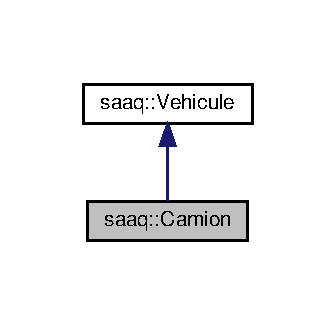
\includegraphics[width=161pt]{classsaaq_1_1Camion__inherit__graph}
\end{center}
\end{figure}


Collaboration diagram for saaq\+:\+:Camion\+:\nopagebreak
\begin{figure}[H]
\begin{center}
\leavevmode
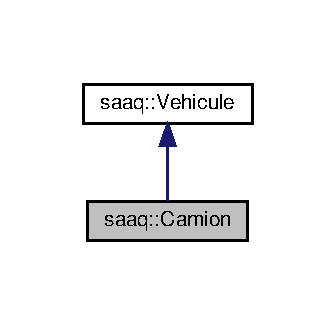
\includegraphics[width=161pt]{classsaaq_1_1Camion__coll__graph}
\end{center}
\end{figure}
\subsection*{Public Member Functions}
\begin{DoxyCompactItemize}
\item 
\hyperlink{classsaaq_1_1Camion_ab81877c7ca4c636c4488c09a6b7fabba}{Camion} (const int p\+\_\+poids, const int p\+\_\+nb\+Essieux, const std\+::string \&p\+\_\+niv, const std\+::string p\+\_\+immatriculation, \hyperlink{classutil_1_1Date}{util\+::\+Date} \&p\+\_\+date\+Enregistrement)
\begin{DoxyCompactList}\small\item\em Constructeur d\textquotesingle{}un nouvel objet de la classe \hyperlink{classsaaq_1_1Camion}{Camion}. \end{DoxyCompactList}\item 
const int \hyperlink{classsaaq_1_1Camion_ab024fec200c2aa4484645da93155cdd2}{req\+Poids} () const
\begin{DoxyCompactList}\small\item\em Retourne le poid du camion. \end{DoxyCompactList}\item 
const int \hyperlink{classsaaq_1_1Camion_aeac12d82162c95755096025f93c8ddb7}{req\+\_\+\+Nb\+Essieux} () const
\begin{DoxyCompactList}\small\item\em Retourne le nombre d\textquotesingle{}essieux du camion. \end{DoxyCompactList}\item 
double \hyperlink{classsaaq_1_1Camion_af01bdc48db3cdeb3bc29c8b864ffdad8}{tarification\+Annuelle} () const
\begin{DoxyCompactList}\small\item\em Retourne la tarification annuelle du camion. \end{DoxyCompactList}\item 
void \hyperlink{classsaaq_1_1Camion_aff39f0171afe70b4a9168ebefba775b5}{asg\+Immatriculation} (const std\+::string \&p\+\_\+immatriculation)
\begin{DoxyCompactList}\small\item\em Assigne une nouvelle plaque automobile au camion. \end{DoxyCompactList}\item 
virtual \hyperlink{classsaaq_1_1Vehicule}{Vehicule} $\ast$ \hyperlink{classsaaq_1_1Camion_aa4fe639e82878acf3fe578a8d80870d4}{clone} () const
\begin{DoxyCompactList}\small\item\em Retourne un clone de l\textquotesingle{}objet du camion. \end{DoxyCompactList}\item 
virtual std\+::string \hyperlink{classsaaq_1_1Camion_a7e352c9d011c145497fa19d16482bd9a}{req\+Vehicule\+Formate} () const
\begin{DoxyCompactList}\small\item\em Retourne une string contenant les informations du camion de maniere formate. \end{DoxyCompactList}\end{DoxyCompactItemize}
\subsection*{Additional Inherited Members}


\subsection{Detailed Description}
Classe \hyperlink{classsaaq_1_1Camion}{Camion} qui contient les informations sur un \hyperlink{classsaaq_1_1Camion}{Camion} Contient la plaque d\textquotesingle{}immatriculation, la date d\textquotesingle{}enregistrement, le poid, le nombre d\textquotesingle{}essieu et le N\+IV du camion. Des méthode qui permettent de nous donner chaques valeurs. Une méthode qui permet d\textquotesingle{}assigner une nouvelle plaque de camion. Une méthode qui permet d\textquotesingle{}afficher le tout dans un format console. 

\subsection{Constructor \& Destructor Documentation}
\mbox{\Hypertarget{classsaaq_1_1Camion_ab81877c7ca4c636c4488c09a6b7fabba}\label{classsaaq_1_1Camion_ab81877c7ca4c636c4488c09a6b7fabba}} 
\index{saaq\+::\+Camion@{saaq\+::\+Camion}!Camion@{Camion}}
\index{Camion@{Camion}!saaq\+::\+Camion@{saaq\+::\+Camion}}
\subsubsection{\texorpdfstring{Camion()}{Camion()}}
{\footnotesize\ttfamily saaq\+::\+Camion\+::\+Camion (\begin{DoxyParamCaption}\item[{const int}]{p\+\_\+poids,  }\item[{const int}]{p\+\_\+nb\+Essieux,  }\item[{const std\+::string \&}]{p\+\_\+niv,  }\item[{const std\+::string}]{p\+\_\+immatriculation,  }\item[{\hyperlink{classutil_1_1Date}{util\+::\+Date} \&}]{p\+\_\+date\+Enregistrement }\end{DoxyParamCaption})}



Constructeur d\textquotesingle{}un nouvel objet de la classe \hyperlink{classsaaq_1_1Camion}{Camion}. 


\begin{DoxyParams}[1]{Parameters}
\mbox{\tt in}  & {\em p\+\_\+poids} & poid du camion \\
\hline
\mbox{\tt in}  & {\em p\+\_\+nb\+Essieux} & nombre d\textquotesingle{}essieux \\
\hline
\mbox{\tt in}  & {\em p\+\_\+niv} & N\+IV du vehicule \\
\hline
\mbox{\tt in}  & {\em p\+\_\+immatriculation} & immatriculation du vehicule \\
\hline
\mbox{\tt in}  & {\em p\+\_\+date\+Enregistrement} & date d\textquotesingle{}enregistrement \\
\hline
\end{DoxyParams}
\begin{DoxyPrecond}{Precondition}
p\+\_\+immatriculation est une plaque de camion 

p\+\_\+poids est valide (plus grand que 3000) 

p\+\_\+nb\+Essieux est valide (plus que 2 essieux) 
\end{DoxyPrecond}
\begin{DoxyPostcond}{Postcondition}
m\+\_\+poids prend la valeur de p\+\_\+poids 

m\+\_\+nb\+Essieux prend la valeur de p\+\_\+nb\+Essieux 
\end{DoxyPostcond}


\subsection{Member Function Documentation}
\mbox{\Hypertarget{classsaaq_1_1Camion_aff39f0171afe70b4a9168ebefba775b5}\label{classsaaq_1_1Camion_aff39f0171afe70b4a9168ebefba775b5}} 
\index{saaq\+::\+Camion@{saaq\+::\+Camion}!asg\+Immatriculation@{asg\+Immatriculation}}
\index{asg\+Immatriculation@{asg\+Immatriculation}!saaq\+::\+Camion@{saaq\+::\+Camion}}
\subsubsection{\texorpdfstring{asg\+Immatriculation()}{asgImmatriculation()}}
{\footnotesize\ttfamily void saaq\+::\+Camion\+::asg\+Immatriculation (\begin{DoxyParamCaption}\item[{const std\+::string \&}]{p\+\_\+immatriculation }\end{DoxyParamCaption})}



Assigne une nouvelle plaque automobile au camion. 


\begin{DoxyParams}[1]{Parameters}
\mbox{\tt in}  & {\em p\+\_\+immatriculation} & est la nouvelle plaque du camion qui est valide \\
\hline
\end{DoxyParams}
\begin{DoxyPrecond}{Precondition}
p\+\_\+immatriculation correspond a une plaque automobile valide 
\end{DoxyPrecond}
\begin{DoxyPostcond}{Postcondition}
la nouvelle plaque a été assigné correctement 
\end{DoxyPostcond}
\mbox{\Hypertarget{classsaaq_1_1Camion_aa4fe639e82878acf3fe578a8d80870d4}\label{classsaaq_1_1Camion_aa4fe639e82878acf3fe578a8d80870d4}} 
\index{saaq\+::\+Camion@{saaq\+::\+Camion}!clone@{clone}}
\index{clone@{clone}!saaq\+::\+Camion@{saaq\+::\+Camion}}
\subsubsection{\texorpdfstring{clone()}{clone()}}
{\footnotesize\ttfamily \hyperlink{classsaaq_1_1Vehicule}{Vehicule} $\ast$ saaq\+::\+Camion\+::clone (\begin{DoxyParamCaption}{ }\end{DoxyParamCaption}) const\hspace{0.3cm}{\ttfamily [virtual]}}



Retourne un clone de l\textquotesingle{}objet du camion. 

\begin{DoxyReturn}{Returns}
une copie du camion 
\end{DoxyReturn}


Implements \hyperlink{classsaaq_1_1Vehicule}{saaq\+::\+Vehicule}.

\mbox{\Hypertarget{classsaaq_1_1Camion_aeac12d82162c95755096025f93c8ddb7}\label{classsaaq_1_1Camion_aeac12d82162c95755096025f93c8ddb7}} 
\index{saaq\+::\+Camion@{saaq\+::\+Camion}!req\+\_\+\+Nb\+Essieux@{req\+\_\+\+Nb\+Essieux}}
\index{req\+\_\+\+Nb\+Essieux@{req\+\_\+\+Nb\+Essieux}!saaq\+::\+Camion@{saaq\+::\+Camion}}
\subsubsection{\texorpdfstring{req\+\_\+\+Nb\+Essieux()}{req\_NbEssieux()}}
{\footnotesize\ttfamily const int saaq\+::\+Camion\+::req\+\_\+\+Nb\+Essieux (\begin{DoxyParamCaption}{ }\end{DoxyParamCaption}) const}



Retourne le nombre d\textquotesingle{}essieux du camion. 

\begin{DoxyReturn}{Returns}
le nombre d\textquotesingle{}essieux 
\end{DoxyReturn}
\mbox{\Hypertarget{classsaaq_1_1Camion_ab024fec200c2aa4484645da93155cdd2}\label{classsaaq_1_1Camion_ab024fec200c2aa4484645da93155cdd2}} 
\index{saaq\+::\+Camion@{saaq\+::\+Camion}!req\+Poids@{req\+Poids}}
\index{req\+Poids@{req\+Poids}!saaq\+::\+Camion@{saaq\+::\+Camion}}
\subsubsection{\texorpdfstring{req\+Poids()}{reqPoids()}}
{\footnotesize\ttfamily const int saaq\+::\+Camion\+::req\+Poids (\begin{DoxyParamCaption}{ }\end{DoxyParamCaption}) const}



Retourne le poid du camion. 

\begin{DoxyReturn}{Returns}
poid du camion 
\end{DoxyReturn}
\mbox{\Hypertarget{classsaaq_1_1Camion_a7e352c9d011c145497fa19d16482bd9a}\label{classsaaq_1_1Camion_a7e352c9d011c145497fa19d16482bd9a}} 
\index{saaq\+::\+Camion@{saaq\+::\+Camion}!req\+Vehicule\+Formate@{req\+Vehicule\+Formate}}
\index{req\+Vehicule\+Formate@{req\+Vehicule\+Formate}!saaq\+::\+Camion@{saaq\+::\+Camion}}
\subsubsection{\texorpdfstring{req\+Vehicule\+Formate()}{reqVehiculeFormate()}}
{\footnotesize\ttfamily std\+::string saaq\+::\+Camion\+::req\+Vehicule\+Formate (\begin{DoxyParamCaption}{ }\end{DoxyParamCaption}) const\hspace{0.3cm}{\ttfamily [virtual]}}



Retourne une string contenant les informations du camion de maniere formate. 

\begin{DoxyReturn}{Returns}
informations du camion de maniere formate 
\end{DoxyReturn}


Reimplemented from \hyperlink{classsaaq_1_1Vehicule_a9d0ff95273ecd7858cf9bd12aac359ba}{saaq\+::\+Vehicule}.

\mbox{\Hypertarget{classsaaq_1_1Camion_af01bdc48db3cdeb3bc29c8b864ffdad8}\label{classsaaq_1_1Camion_af01bdc48db3cdeb3bc29c8b864ffdad8}} 
\index{saaq\+::\+Camion@{saaq\+::\+Camion}!tarification\+Annuelle@{tarification\+Annuelle}}
\index{tarification\+Annuelle@{tarification\+Annuelle}!saaq\+::\+Camion@{saaq\+::\+Camion}}
\subsubsection{\texorpdfstring{tarification\+Annuelle()}{tarificationAnnuelle()}}
{\footnotesize\ttfamily double saaq\+::\+Camion\+::tarification\+Annuelle (\begin{DoxyParamCaption}{ }\end{DoxyParamCaption}) const\hspace{0.3cm}{\ttfamily [virtual]}}



Retourne la tarification annuelle du camion. 

\begin{DoxyReturn}{Returns}
tarification annuelle du camion 
\end{DoxyReturn}


Implements \hyperlink{classsaaq_1_1Vehicule_a93570921069d25b6bc48cf04af176395}{saaq\+::\+Vehicule}.



The documentation for this class was generated from the following files\+:\begin{DoxyCompactItemize}
\item 
\hyperlink{Camion_8h}{Camion.\+h}\item 
\hyperlink{Camion_8cpp}{Camion.\+cpp}\end{DoxyCompactItemize}

\hypertarget{classContratException}{}\section{Contrat\+Exception Class Reference}
\label{classContratException}\index{Contrat\+Exception@{Contrat\+Exception}}


Classe de base des exceptions de contrat.  




{\ttfamily \#include $<$Contrat\+Exception.\+h$>$}



Inheritance diagram for Contrat\+Exception\+:\nopagebreak
\begin{figure}[H]
\begin{center}
\leavevmode
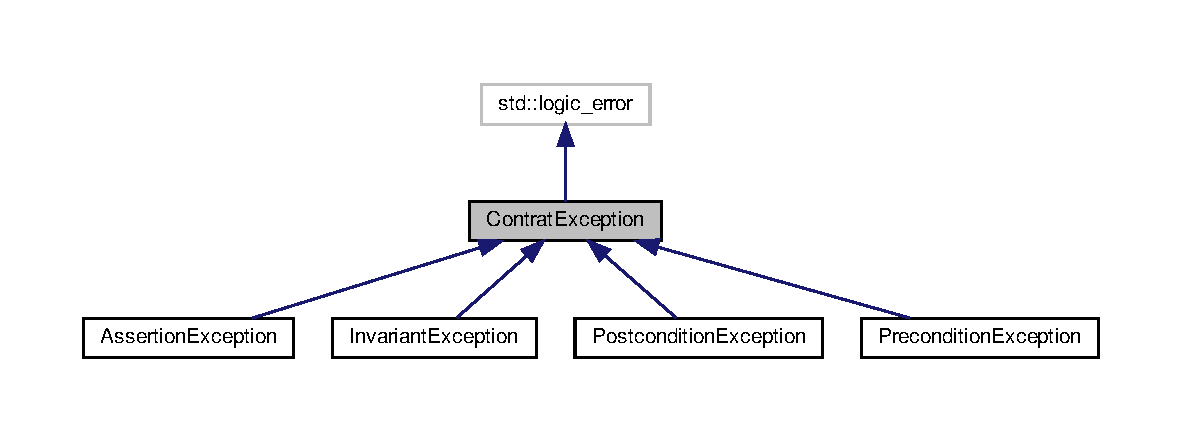
\includegraphics[width=350pt]{classContratException__inherit__graph}
\end{center}
\end{figure}


Collaboration diagram for Contrat\+Exception\+:\nopagebreak
\begin{figure}[H]
\begin{center}
\leavevmode
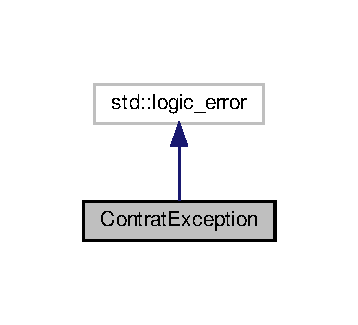
\includegraphics[width=172pt]{classContratException__coll__graph}
\end{center}
\end{figure}
\subsection*{Public Member Functions}
\begin{DoxyCompactItemize}
\item 
\hyperlink{classContratException_ad6c04fb577e960f87e010b125aa636a0}{Contrat\+Exception} (std\+::string, unsigned int, std\+::string, std\+::string)
\begin{DoxyCompactList}\small\item\em Constructeur de la classe de base \hyperlink{classContratException}{Contrat\+Exception}. \end{DoxyCompactList}\item 
std\+::string \hyperlink{classContratException_a59c9ed58985dcdd70af4ee50b2937707}{req\+Texte\+Exception} () const
\begin{DoxyCompactList}\small\item\em Construit le texte complet relié à l\textquotesingle{}exception de contrat. \end{DoxyCompactList}\end{DoxyCompactItemize}


\subsection{Detailed Description}
Classe de base des exceptions de contrat. 

\subsection{Constructor \& Destructor Documentation}
\mbox{\Hypertarget{classContratException_ad6c04fb577e960f87e010b125aa636a0}\label{classContratException_ad6c04fb577e960f87e010b125aa636a0}} 
\index{Contrat\+Exception@{Contrat\+Exception}!Contrat\+Exception@{Contrat\+Exception}}
\index{Contrat\+Exception@{Contrat\+Exception}!Contrat\+Exception@{Contrat\+Exception}}
\subsubsection{\texorpdfstring{Contrat\+Exception()}{ContratException()}}
{\footnotesize\ttfamily Contrat\+Exception\+::\+Contrat\+Exception (\begin{DoxyParamCaption}\item[{std\+::string}]{p\+\_\+fichP,  }\item[{unsigned int}]{p\+\_\+prm\+Ligne,  }\item[{std\+::string}]{p\+\_\+exprP,  }\item[{std\+::string}]{p\+\_\+msgP }\end{DoxyParamCaption})}



Constructeur de la classe de base \hyperlink{classContratException}{Contrat\+Exception}. 


\begin{DoxyParams}{Parameters}
{\em p\+\_\+fichP} & chaîne de caractères représentant le fichier source dans lequel a eu lieu l\textquotesingle{}erreur \\
\hline
{\em p\+\_\+prm\+Ligne} & un entier représentant la ligne où a eu lieu l\textquotesingle{}erreur \\
\hline
{\em p\+\_\+msgP} & Message décrivant l\textquotesingle{}erreur \\
\hline
{\em p\+\_\+exprP} & Test logique qui a échoué \\
\hline
\end{DoxyParams}


\subsection{Member Function Documentation}
\mbox{\Hypertarget{classContratException_a59c9ed58985dcdd70af4ee50b2937707}\label{classContratException_a59c9ed58985dcdd70af4ee50b2937707}} 
\index{Contrat\+Exception@{Contrat\+Exception}!req\+Texte\+Exception@{req\+Texte\+Exception}}
\index{req\+Texte\+Exception@{req\+Texte\+Exception}!Contrat\+Exception@{Contrat\+Exception}}
\subsubsection{\texorpdfstring{req\+Texte\+Exception()}{reqTexteException()}}
{\footnotesize\ttfamily std\+::string Contrat\+Exception\+::req\+Texte\+Exception (\begin{DoxyParamCaption}{ }\end{DoxyParamCaption}) const}



Construit le texte complet relié à l\textquotesingle{}exception de contrat. 

\begin{DoxyReturn}{Returns}
une chaîne de caractères correspondant à l\textquotesingle{}exception 
\end{DoxyReturn}


The documentation for this class was generated from the following files\+:\begin{DoxyCompactItemize}
\item 
\hyperlink{ContratException_8h}{Contrat\+Exception.\+h}\item 
\hyperlink{ContratException_8cpp}{Contrat\+Exception.\+cpp}\end{DoxyCompactItemize}

\hypertarget{classutil_1_1Date}{}\section{util\+:\+:Date Class Reference}
\label{classutil_1_1Date}\index{util\+::\+Date@{util\+::\+Date}}


Cette classe sert au maintien et à la manipulation des dates.  




{\ttfamily \#include $<$Date.\+h$>$}

\subsection*{Public Member Functions}
\begin{DoxyCompactItemize}
\item 
\mbox{\Hypertarget{classutil_1_1Date_a03f7ca00aa80f113bc7c0ebfbd769f54}\label{classutil_1_1Date_a03f7ca00aa80f113bc7c0ebfbd769f54}} 
\hyperlink{classutil_1_1Date_a03f7ca00aa80f113bc7c0ebfbd769f54}{Date} ()
\begin{DoxyCompactList}\small\item\em constructeur par défaut ~\newline
La date prise par défaut est la date du système \end{DoxyCompactList}\item 
\hyperlink{classutil_1_1Date_a06b8340e5beed84c885c89d41a750330}{Date} (long p\+\_\+jour, long p\+\_\+mois, long p\+\_\+annee)
\begin{DoxyCompactList}\small\item\em constructeur avec paramètres On construit un objet \hyperlink{classutil_1_1Date}{Date} à partir de valeurs passées en paramètres. \end{DoxyCompactList}\item 
void \hyperlink{classutil_1_1Date_ab82f59d834f60b929ca130f15e5279c3}{asg\+Date} (long p\+\_\+jour, long p\+\_\+mois, long p\+\_\+annee)
\begin{DoxyCompactList}\small\item\em Assigne une date à l\textquotesingle{}objet courant. \end{DoxyCompactList}\item 
bool \hyperlink{classutil_1_1Date_a7788599612a71d89126d649fdaaced3d}{ajoute\+Nb\+Jour} (long p\+\_\+nbjour)
\begin{DoxyCompactList}\small\item\em Ajoute ou retire un certain nombre de jours à la date courante. \end{DoxyCompactList}\item 
long \hyperlink{classutil_1_1Date_aa2b8c7a6e23e9244a5bac8342484d3b8}{req\+Jour} () const
\begin{DoxyCompactList}\small\item\em retourne le jour de la date \end{DoxyCompactList}\item 
long \hyperlink{classutil_1_1Date_a8002c391b812945da68b16cb4a424460}{req\+Mois} () const
\begin{DoxyCompactList}\small\item\em retourne le mois de la date \end{DoxyCompactList}\item 
long \hyperlink{classutil_1_1Date_aa7c4b428456da55a2e3769e93ad9bb8d}{req\+Annee} () const
\begin{DoxyCompactList}\small\item\em retourne l\textquotesingle{}année de la date \end{DoxyCompactList}\item 
long \hyperlink{classutil_1_1Date_a9e76af410b6be9ac4ea9ab4df5797847}{req\+Jour\+Annee} () const
\begin{DoxyCompactList}\small\item\em retourne le numéro correspondant au jour de la date \end{DoxyCompactList}\item 
std\+::string \hyperlink{classutil_1_1Date_ad92d1e9c4d570c5f31a8e06cf2e1ae8c}{req\+Date\+Formatee} () const
\begin{DoxyCompactList}\small\item\em retourne une date formatée dans une chaîne de caracères (string) \end{DoxyCompactList}\item 
bool \hyperlink{classutil_1_1Date_a8114f8e40cee24e1d7a58b910e8f4637}{operator==} (const \hyperlink{classutil_1_1Date}{Date} \&p\+\_\+date) const
\begin{DoxyCompactList}\small\item\em surcharge de l\textquotesingle{}opérateur == \end{DoxyCompactList}\item 
bool \hyperlink{classutil_1_1Date_aefcf8a7520711f783fb0241d460480c5}{operator$<$} (const \hyperlink{classutil_1_1Date}{Date} \&p\+\_\+date) const
\begin{DoxyCompactList}\small\item\em surcharge de l\textquotesingle{}opérateur $<$ \end{DoxyCompactList}\item 
int \hyperlink{classutil_1_1Date_af12f2c545070b5e2b397be5379c5c3fd}{operator-\/} (const \hyperlink{classutil_1_1Date}{Date} \&p\+\_\+date) const
\begin{DoxyCompactList}\small\item\em retourne le nombre de jours entre deux dates \end{DoxyCompactList}\end{DoxyCompactItemize}
\subsection*{Static Public Member Functions}
\begin{DoxyCompactItemize}
\item 
static bool \hyperlink{classutil_1_1Date_af80efec6a713cdb671d8b23c3e8c4efb}{est\+Bissextile} (long p\+\_\+annee)
\begin{DoxyCompactList}\small\item\em Déterminer si une année est bissextile ou non. \end{DoxyCompactList}\item 
static bool \hyperlink{classutil_1_1Date_af4b4dde01395754245a42483358cb538}{valider\+Date} (long p\+\_\+jour, long p\+\_\+mois, long p\+\_\+annee)
\begin{DoxyCompactList}\small\item\em Vérifie la validité d\textquotesingle{}une date. \end{DoxyCompactList}\end{DoxyCompactItemize}
\subsection*{Friends}
\begin{DoxyCompactItemize}
\item 
\mbox{\Hypertarget{classutil_1_1Date_ab01372aff5a2aa1d5f5bab251bb7951c}\label{classutil_1_1Date_ab01372aff5a2aa1d5f5bab251bb7951c}} 
std\+::ostream \& {\bfseries operator$<$$<$} (std\+::ostream \&p\+\_\+os, const \hyperlink{classutil_1_1Date}{Date} \&p\+\_\+date)
\end{DoxyCompactItemize}


\subsection{Detailed Description}
Cette classe sert au maintien et à la manipulation des dates. 

Cette classe peut aussi servir à prendre la date courante du système et à faire des calculs avec des dates. 

Les limites de validité de cette date est du 1er janvier 1970 au 31 décembre 2037. 

La validité d\textquotesingle{}une date peut être vérifiée avec la méthode statique bool Date\+::verifier\+Date(jour, mois, annee).~\newline
 Attributs\+: time\+\_\+t m\+\_\+temps Nombre de secondes écoulé depuis le premier janvier 1970 time\+\_\+t m\+\_\+temps pour long m\+\_\+temps 

\subsection{Constructor \& Destructor Documentation}
\mbox{\Hypertarget{classutil_1_1Date_a06b8340e5beed84c885c89d41a750330}\label{classutil_1_1Date_a06b8340e5beed84c885c89d41a750330}} 
\index{util\+::\+Date@{util\+::\+Date}!Date@{Date}}
\index{Date@{Date}!util\+::\+Date@{util\+::\+Date}}
\subsubsection{\texorpdfstring{Date()}{Date()}}
{\footnotesize\ttfamily util\+::\+Date\+::\+Date (\begin{DoxyParamCaption}\item[{long}]{p\+\_\+jour,  }\item[{long}]{p\+\_\+mois,  }\item[{long}]{p\+\_\+annee }\end{DoxyParamCaption})}



constructeur avec paramètres On construit un objet \hyperlink{classutil_1_1Date}{Date} à partir de valeurs passées en paramètres. 


\begin{DoxyParams}[1]{Parameters}
\mbox{\tt in}  & {\em p\+\_\+jour} & est un entier long qui représente le jour de la date \\
\hline
\mbox{\tt in}  & {\em p\+\_\+mois} & est un entier long qui représente le mois de la date \\
\hline
\mbox{\tt in}  & {\em p\+\_\+annee} & est un entier long qui représente l\textquotesingle{}année de la date \\
\hline
\end{DoxyParams}


\subsection{Member Function Documentation}
\mbox{\Hypertarget{classutil_1_1Date_a7788599612a71d89126d649fdaaced3d}\label{classutil_1_1Date_a7788599612a71d89126d649fdaaced3d}} 
\index{util\+::\+Date@{util\+::\+Date}!ajoute\+Nb\+Jour@{ajoute\+Nb\+Jour}}
\index{ajoute\+Nb\+Jour@{ajoute\+Nb\+Jour}!util\+::\+Date@{util\+::\+Date}}
\subsubsection{\texorpdfstring{ajoute\+Nb\+Jour()}{ajouteNbJour()}}
{\footnotesize\ttfamily bool util\+::\+Date\+::ajoute\+Nb\+Jour (\begin{DoxyParamCaption}\item[{long}]{p\+\_\+nb\+Jour }\end{DoxyParamCaption})}



Ajoute ou retire un certain nombre de jours à la date courante. 


\begin{DoxyParams}[1]{Parameters}
\mbox{\tt in}  & {\em p\+\_\+nb\+Jour} & est une entier long qui représente le nombre de jours à ajouter ou à soustraire s\textquotesingle{}il est négatif \\
\hline
\end{DoxyParams}
\begin{DoxyReturn}{Returns}
un booléen qui indique si l\textquotesingle{}opération a réussi ou non 
\end{DoxyReturn}
\mbox{\Hypertarget{classutil_1_1Date_ab82f59d834f60b929ca130f15e5279c3}\label{classutil_1_1Date_ab82f59d834f60b929ca130f15e5279c3}} 
\index{util\+::\+Date@{util\+::\+Date}!asg\+Date@{asg\+Date}}
\index{asg\+Date@{asg\+Date}!util\+::\+Date@{util\+::\+Date}}
\subsubsection{\texorpdfstring{asg\+Date()}{asgDate()}}
{\footnotesize\ttfamily void util\+::\+Date\+::asg\+Date (\begin{DoxyParamCaption}\item[{long}]{p\+\_\+jour,  }\item[{long}]{p\+\_\+mois,  }\item[{long}]{p\+\_\+annee }\end{DoxyParamCaption})}



Assigne une date à l\textquotesingle{}objet courant. 


\begin{DoxyParams}[1]{Parameters}
\mbox{\tt in}  & {\em p\+\_\+jour} & est un entier long qui représente le jour de la date \\
\hline
\mbox{\tt in}  & {\em p\+\_\+mois} & est un entier long qui représente le mois de la date \\
\hline
\mbox{\tt in}  & {\em p\+\_\+annee} & est un entier long qui représente l\textquotesingle{}année de la date \\
\hline
\end{DoxyParams}
\mbox{\Hypertarget{classutil_1_1Date_af80efec6a713cdb671d8b23c3e8c4efb}\label{classutil_1_1Date_af80efec6a713cdb671d8b23c3e8c4efb}} 
\index{util\+::\+Date@{util\+::\+Date}!est\+Bissextile@{est\+Bissextile}}
\index{est\+Bissextile@{est\+Bissextile}!util\+::\+Date@{util\+::\+Date}}
\subsubsection{\texorpdfstring{est\+Bissextile()}{estBissextile()}}
{\footnotesize\ttfamily bool util\+::\+Date\+::est\+Bissextile (\begin{DoxyParamCaption}\item[{long}]{p\+\_\+annee }\end{DoxyParamCaption})\hspace{0.3cm}{\ttfamily [static]}}



Déterminer si une année est bissextile ou non. 


\begin{DoxyParams}[1]{Parameters}
\mbox{\tt in}  & {\em p\+\_\+annee} & un entier long qui repréente l\textquotesingle{}année à vérifier \\
\hline
\end{DoxyParams}
\begin{DoxyReturn}{Returns}
est\+Bissextile un booléen qui a la valeur true si l\textquotesingle{}année est bissextile et false sinon 
\end{DoxyReturn}
\mbox{\Hypertarget{classutil_1_1Date_af12f2c545070b5e2b397be5379c5c3fd}\label{classutil_1_1Date_af12f2c545070b5e2b397be5379c5c3fd}} 
\index{util\+::\+Date@{util\+::\+Date}!operator-\/@{operator-\/}}
\index{operator-\/@{operator-\/}!util\+::\+Date@{util\+::\+Date}}
\subsubsection{\texorpdfstring{operator-\/()}{operator-()}}
{\footnotesize\ttfamily int util\+::\+Date\+::operator-\/ (\begin{DoxyParamCaption}\item[{const \hyperlink{classutil_1_1Date}{Date} \&}]{p\+\_\+date }\end{DoxyParamCaption}) const}



retourne le nombre de jours entre deux dates 


\begin{DoxyParams}[1]{Parameters}
\mbox{\tt in}  & {\em p\+\_\+date} & qui est une date valide \\
\hline
\end{DoxyParams}
\begin{DoxyReturn}{Returns}
un entier qui représente le nombre de jours entre les deux dates 
\end{DoxyReturn}
\mbox{\Hypertarget{classutil_1_1Date_aefcf8a7520711f783fb0241d460480c5}\label{classutil_1_1Date_aefcf8a7520711f783fb0241d460480c5}} 
\index{util\+::\+Date@{util\+::\+Date}!operator$<$@{operator$<$}}
\index{operator$<$@{operator$<$}!util\+::\+Date@{util\+::\+Date}}
\subsubsection{\texorpdfstring{operator$<$()}{operator<()}}
{\footnotesize\ttfamily bool util\+::\+Date\+::operator$<$ (\begin{DoxyParamCaption}\item[{const \hyperlink{classutil_1_1Date}{Date} \&}]{p\+\_\+date }\end{DoxyParamCaption}) const}



surcharge de l\textquotesingle{}opérateur $<$ 


\begin{DoxyParams}[1]{Parameters}
\mbox{\tt in}  & {\em p\+\_\+date} & qui est une date valide \\
\hline
\end{DoxyParams}
\begin{DoxyReturn}{Returns}
un booléen indiquant si la date passée en paramètre est plus petite que la date courante 
\end{DoxyReturn}
\mbox{\Hypertarget{classutil_1_1Date_a8114f8e40cee24e1d7a58b910e8f4637}\label{classutil_1_1Date_a8114f8e40cee24e1d7a58b910e8f4637}} 
\index{util\+::\+Date@{util\+::\+Date}!operator==@{operator==}}
\index{operator==@{operator==}!util\+::\+Date@{util\+::\+Date}}
\subsubsection{\texorpdfstring{operator==()}{operator==()}}
{\footnotesize\ttfamily bool util\+::\+Date\+::operator== (\begin{DoxyParamCaption}\item[{const \hyperlink{classutil_1_1Date}{Date} \&}]{p\+\_\+date }\end{DoxyParamCaption}) const}



surcharge de l\textquotesingle{}opérateur == 


\begin{DoxyParams}[1]{Parameters}
\mbox{\tt in}  & {\em p\+\_\+date} & qui est une date valide \\
\hline
\end{DoxyParams}
\begin{DoxyReturn}{Returns}
un booléen indiquant si les deux dates sont égales ou pas 
\end{DoxyReturn}
\mbox{\Hypertarget{classutil_1_1Date_aa7c4b428456da55a2e3769e93ad9bb8d}\label{classutil_1_1Date_aa7c4b428456da55a2e3769e93ad9bb8d}} 
\index{util\+::\+Date@{util\+::\+Date}!req\+Annee@{req\+Annee}}
\index{req\+Annee@{req\+Annee}!util\+::\+Date@{util\+::\+Date}}
\subsubsection{\texorpdfstring{req\+Annee()}{reqAnnee()}}
{\footnotesize\ttfamily long util\+::\+Date\+::req\+Annee (\begin{DoxyParamCaption}{ }\end{DoxyParamCaption}) const}



retourne l\textquotesingle{}année de la date 

\begin{DoxyReturn}{Returns}
un entier long qui représente l\textquotesingle{}année de la date 
\end{DoxyReturn}
\mbox{\Hypertarget{classutil_1_1Date_ad92d1e9c4d570c5f31a8e06cf2e1ae8c}\label{classutil_1_1Date_ad92d1e9c4d570c5f31a8e06cf2e1ae8c}} 
\index{util\+::\+Date@{util\+::\+Date}!req\+Date\+Formatee@{req\+Date\+Formatee}}
\index{req\+Date\+Formatee@{req\+Date\+Formatee}!util\+::\+Date@{util\+::\+Date}}
\subsubsection{\texorpdfstring{req\+Date\+Formatee()}{reqDateFormatee()}}
{\footnotesize\ttfamily string util\+::\+Date\+::req\+Date\+Formatee (\begin{DoxyParamCaption}{ }\end{DoxyParamCaption}) const}



retourne une date formatée dans une chaîne de caracères (string) 

\begin{DoxyReturn}{Returns}
une date formatée dans une chaîne de caractères 
\end{DoxyReturn}
\mbox{\Hypertarget{classutil_1_1Date_aa2b8c7a6e23e9244a5bac8342484d3b8}\label{classutil_1_1Date_aa2b8c7a6e23e9244a5bac8342484d3b8}} 
\index{util\+::\+Date@{util\+::\+Date}!req\+Jour@{req\+Jour}}
\index{req\+Jour@{req\+Jour}!util\+::\+Date@{util\+::\+Date}}
\subsubsection{\texorpdfstring{req\+Jour()}{reqJour()}}
{\footnotesize\ttfamily long util\+::\+Date\+::req\+Jour (\begin{DoxyParamCaption}{ }\end{DoxyParamCaption}) const}



retourne le jour de la date 

\begin{DoxyReturn}{Returns}
un entier long qui représente le jour de la date 
\end{DoxyReturn}
\mbox{\Hypertarget{classutil_1_1Date_a9e76af410b6be9ac4ea9ab4df5797847}\label{classutil_1_1Date_a9e76af410b6be9ac4ea9ab4df5797847}} 
\index{util\+::\+Date@{util\+::\+Date}!req\+Jour\+Annee@{req\+Jour\+Annee}}
\index{req\+Jour\+Annee@{req\+Jour\+Annee}!util\+::\+Date@{util\+::\+Date}}
\subsubsection{\texorpdfstring{req\+Jour\+Annee()}{reqJourAnnee()}}
{\footnotesize\ttfamily long util\+::\+Date\+::req\+Jour\+Annee (\begin{DoxyParamCaption}{ }\end{DoxyParamCaption}) const}



retourne le numéro correspondant au jour de la date 

\begin{DoxyReturn}{Returns}
un entier long qui représente le numéro correspondant au jour de la date 
\end{DoxyReturn}
\mbox{\Hypertarget{classutil_1_1Date_a8002c391b812945da68b16cb4a424460}\label{classutil_1_1Date_a8002c391b812945da68b16cb4a424460}} 
\index{util\+::\+Date@{util\+::\+Date}!req\+Mois@{req\+Mois}}
\index{req\+Mois@{req\+Mois}!util\+::\+Date@{util\+::\+Date}}
\subsubsection{\texorpdfstring{req\+Mois()}{reqMois()}}
{\footnotesize\ttfamily long util\+::\+Date\+::req\+Mois (\begin{DoxyParamCaption}{ }\end{DoxyParamCaption}) const}



retourne le mois de la date 

\begin{DoxyReturn}{Returns}
un entier long qui représente le mois de la date 
\end{DoxyReturn}
\mbox{\Hypertarget{classutil_1_1Date_af4b4dde01395754245a42483358cb538}\label{classutil_1_1Date_af4b4dde01395754245a42483358cb538}} 
\index{util\+::\+Date@{util\+::\+Date}!valider\+Date@{valider\+Date}}
\index{valider\+Date@{valider\+Date}!util\+::\+Date@{util\+::\+Date}}
\subsubsection{\texorpdfstring{valider\+Date()}{validerDate()}}
{\footnotesize\ttfamily bool util\+::\+Date\+::valider\+Date (\begin{DoxyParamCaption}\item[{long}]{p\+\_\+jour,  }\item[{long}]{p\+\_\+mois,  }\item[{long}]{p\+\_\+annee }\end{DoxyParamCaption})\hspace{0.3cm}{\ttfamily [static]}}



Vérifie la validité d\textquotesingle{}une date. 


\begin{DoxyParams}[1]{Parameters}
\mbox{\tt in}  & {\em p\+\_\+jour} & un entier long représentant le jour de la date \\
\hline
\mbox{\tt in}  & {\em p\+\_\+mois} & un entier long représentant le mois de la date \\
\hline
\mbox{\tt in}  & {\em p\+\_\+annee} & un entier long représentant l\textquotesingle{}année de la date \\
\hline
\end{DoxyParams}
\begin{DoxyReturn}{Returns}
un booléen indiquant si la date est valide ou non 
\end{DoxyReturn}


The documentation for this class was generated from the following files\+:\begin{DoxyCompactItemize}
\item 
\hyperlink{Date_8h}{Date.\+h}\item 
\hyperlink{Date_8cpp}{Date.\+cpp}\end{DoxyCompactItemize}

\hypertarget{classInvariantException}{}\section{Invariant\+Exception Class Reference}
\label{classInvariantException}\index{Invariant\+Exception@{Invariant\+Exception}}


Classe pour la gestion des erreurs d\textquotesingle{}invariant.  




{\ttfamily \#include $<$Contrat\+Exception.\+h$>$}



Inheritance diagram for Invariant\+Exception\+:\nopagebreak
\begin{figure}[H]
\begin{center}
\leavevmode
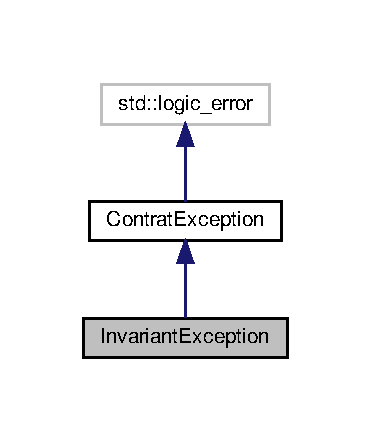
\includegraphics[width=178pt]{classInvariantException__inherit__graph}
\end{center}
\end{figure}


Collaboration diagram for Invariant\+Exception\+:\nopagebreak
\begin{figure}[H]
\begin{center}
\leavevmode
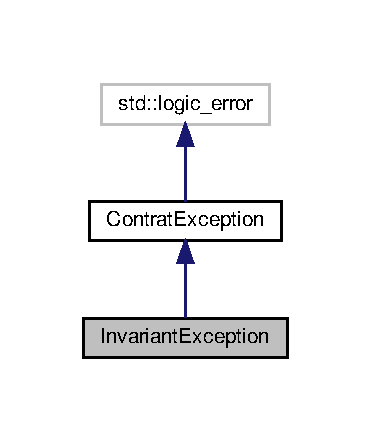
\includegraphics[width=178pt]{classInvariantException__coll__graph}
\end{center}
\end{figure}
\subsection*{Public Member Functions}
\begin{DoxyCompactItemize}
\item 
\hyperlink{classInvariantException_af8a1950834b26c256db0b11eb33e6056}{Invariant\+Exception} (std\+::string, unsigned int, std\+::string)
\begin{DoxyCompactList}\small\item\em Constructeur de la classe \hyperlink{classInvariantException}{Invariant\+Exception} en initialisant la classe de base \hyperlink{classContratException}{Contrat\+Exception}. La classe représente des erreurs d\textquotesingle{}invariant dans la théorie du contrat. \end{DoxyCompactList}\end{DoxyCompactItemize}


\subsection{Detailed Description}
Classe pour la gestion des erreurs d\textquotesingle{}invariant. 

\subsection{Constructor \& Destructor Documentation}
\mbox{\Hypertarget{classInvariantException_af8a1950834b26c256db0b11eb33e6056}\label{classInvariantException_af8a1950834b26c256db0b11eb33e6056}} 
\index{Invariant\+Exception@{Invariant\+Exception}!Invariant\+Exception@{Invariant\+Exception}}
\index{Invariant\+Exception@{Invariant\+Exception}!Invariant\+Exception@{Invariant\+Exception}}
\subsubsection{\texorpdfstring{Invariant\+Exception()}{InvariantException()}}
{\footnotesize\ttfamily Invariant\+Exception\+::\+Invariant\+Exception (\begin{DoxyParamCaption}\item[{std\+::string}]{p\+\_\+fichP,  }\item[{unsigned int}]{p\+\_\+prm\+Ligne,  }\item[{std\+::string}]{p\+\_\+exprP }\end{DoxyParamCaption})}



Constructeur de la classe \hyperlink{classInvariantException}{Invariant\+Exception} en initialisant la classe de base \hyperlink{classContratException}{Contrat\+Exception}. La classe représente des erreurs d\textquotesingle{}invariant dans la théorie du contrat. 


\begin{DoxyParams}{Parameters}
{\em p\+\_\+fichP} & chaîne de caractères représentant le fichier source dans lequel a eu lieu l\textquotesingle{}erreur \\
\hline
{\em p\+\_\+prm\+Ligne} & un entier représentant la ligne où a eu lieu l\textquotesingle{}erreur \\
\hline
{\em p\+\_\+exprP} & Test logique qui a échoué \\
\hline
\end{DoxyParams}


The documentation for this class was generated from the following files\+:\begin{DoxyCompactItemize}
\item 
\hyperlink{ContratException_8h}{Contrat\+Exception.\+h}\item 
\hyperlink{ContratException_8cpp}{Contrat\+Exception.\+cpp}\end{DoxyCompactItemize}

\hypertarget{classPostconditionException}{}\section{Postcondition\+Exception Class Reference}
\label{classPostconditionException}\index{Postcondition\+Exception@{Postcondition\+Exception}}


Classe pour la gestion des erreurs de postcondition.  




{\ttfamily \#include $<$Contrat\+Exception.\+h$>$}



Inheritance diagram for Postcondition\+Exception\+:\nopagebreak
\begin{figure}[H]
\begin{center}
\leavevmode
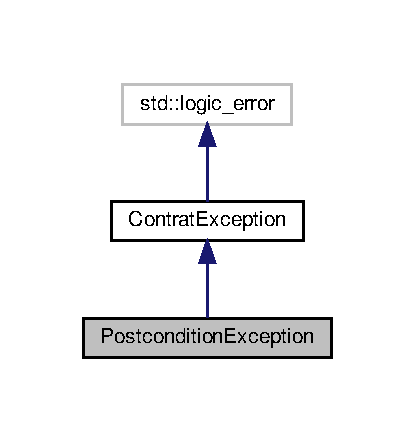
\includegraphics[width=199pt]{classPostconditionException__inherit__graph}
\end{center}
\end{figure}


Collaboration diagram for Postcondition\+Exception\+:\nopagebreak
\begin{figure}[H]
\begin{center}
\leavevmode
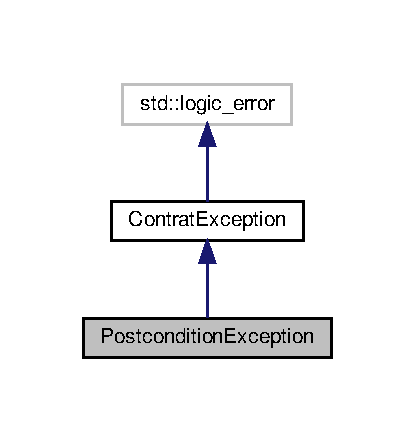
\includegraphics[width=199pt]{classPostconditionException__coll__graph}
\end{center}
\end{figure}
\subsection*{Public Member Functions}
\begin{DoxyCompactItemize}
\item 
\hyperlink{classPostconditionException_acc95ea17c4302b996261b7201d2cf6c4}{Postcondition\+Exception} (std\+::string, unsigned int, std\+::string)
\begin{DoxyCompactList}\small\item\em Constructeur de la classe \hyperlink{classPostconditionException}{Postcondition\+Exception} en initialisant la classe de base \hyperlink{classContratException}{Contrat\+Exception}. La classe représente des erreurs de postcondition dans la théorie du contrat. \end{DoxyCompactList}\end{DoxyCompactItemize}


\subsection{Detailed Description}
Classe pour la gestion des erreurs de postcondition. 

\subsection{Constructor \& Destructor Documentation}
\mbox{\Hypertarget{classPostconditionException_acc95ea17c4302b996261b7201d2cf6c4}\label{classPostconditionException_acc95ea17c4302b996261b7201d2cf6c4}} 
\index{Postcondition\+Exception@{Postcondition\+Exception}!Postcondition\+Exception@{Postcondition\+Exception}}
\index{Postcondition\+Exception@{Postcondition\+Exception}!Postcondition\+Exception@{Postcondition\+Exception}}
\subsubsection{\texorpdfstring{Postcondition\+Exception()}{PostconditionException()}}
{\footnotesize\ttfamily Postcondition\+Exception\+::\+Postcondition\+Exception (\begin{DoxyParamCaption}\item[{std\+::string}]{p\+\_\+fichP,  }\item[{unsigned int}]{p\+\_\+prm\+Ligne,  }\item[{std\+::string}]{p\+\_\+exprP }\end{DoxyParamCaption})}



Constructeur de la classe \hyperlink{classPostconditionException}{Postcondition\+Exception} en initialisant la classe de base \hyperlink{classContratException}{Contrat\+Exception}. La classe représente des erreurs de postcondition dans la théorie du contrat. 


\begin{DoxyParams}{Parameters}
{\em p\+\_\+fichP} & chaîne de caractères représentant le fichier source dans lequel a eu lieu l\textquotesingle{}erreur \\
\hline
{\em p\+\_\+prm\+Ligne} & un entier représentant la ligne où a eu lieu l\textquotesingle{}erreur \\
\hline
{\em p\+\_\+exprP} & Test logique qui a échoué \\
\hline
\end{DoxyParams}


The documentation for this class was generated from the following files\+:\begin{DoxyCompactItemize}
\item 
\hyperlink{ContratException_8h}{Contrat\+Exception.\+h}\item 
\hyperlink{ContratException_8cpp}{Contrat\+Exception.\+cpp}\end{DoxyCompactItemize}

\hypertarget{classPreconditionException}{}\section{Precondition\+Exception Class Reference}
\label{classPreconditionException}\index{Precondition\+Exception@{Precondition\+Exception}}


Classe pour la gestion des erreurs de précondition.  




{\ttfamily \#include $<$Contrat\+Exception.\+h$>$}



Inheritance diagram for Precondition\+Exception\+:\nopagebreak
\begin{figure}[H]
\begin{center}
\leavevmode
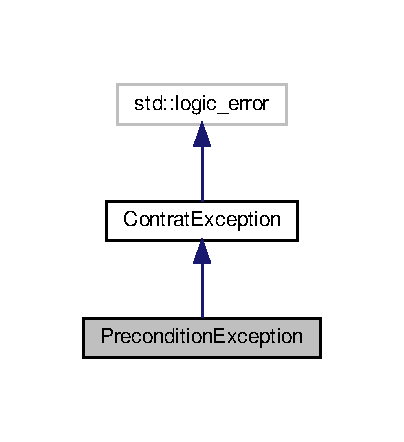
\includegraphics[width=194pt]{classPreconditionException__inherit__graph}
\end{center}
\end{figure}


Collaboration diagram for Precondition\+Exception\+:\nopagebreak
\begin{figure}[H]
\begin{center}
\leavevmode
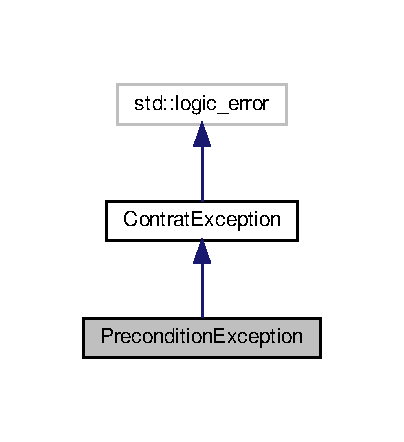
\includegraphics[width=194pt]{classPreconditionException__coll__graph}
\end{center}
\end{figure}
\subsection*{Public Member Functions}
\begin{DoxyCompactItemize}
\item 
\hyperlink{classPreconditionException_a66d4b4c57a0675d487dab85d2c31b08c}{Precondition\+Exception} (std\+::string, unsigned int, std\+::string)
\begin{DoxyCompactList}\small\item\em Constructeur de la classe \hyperlink{classPreconditionException}{Precondition\+Exception} en initialisant la classe de base \hyperlink{classContratException}{Contrat\+Exception}. La classe représente l\textquotesingle{}erreur de précondition dans la théorie du contrat. \end{DoxyCompactList}\end{DoxyCompactItemize}


\subsection{Detailed Description}
Classe pour la gestion des erreurs de précondition. 

\subsection{Constructor \& Destructor Documentation}
\mbox{\Hypertarget{classPreconditionException_a66d4b4c57a0675d487dab85d2c31b08c}\label{classPreconditionException_a66d4b4c57a0675d487dab85d2c31b08c}} 
\index{Precondition\+Exception@{Precondition\+Exception}!Precondition\+Exception@{Precondition\+Exception}}
\index{Precondition\+Exception@{Precondition\+Exception}!Precondition\+Exception@{Precondition\+Exception}}
\subsubsection{\texorpdfstring{Precondition\+Exception()}{PreconditionException()}}
{\footnotesize\ttfamily Precondition\+Exception\+::\+Precondition\+Exception (\begin{DoxyParamCaption}\item[{std\+::string}]{p\+\_\+fichP,  }\item[{unsigned int}]{p\+\_\+prm\+Ligne,  }\item[{std\+::string}]{p\+\_\+exprP }\end{DoxyParamCaption})}



Constructeur de la classe \hyperlink{classPreconditionException}{Precondition\+Exception} en initialisant la classe de base \hyperlink{classContratException}{Contrat\+Exception}. La classe représente l\textquotesingle{}erreur de précondition dans la théorie du contrat. 


\begin{DoxyParams}{Parameters}
{\em p\+\_\+fichP} & chaîne de caractères représentant le fichier source dans lequel a eu lieu l\textquotesingle{}erreur \\
\hline
{\em p\+\_\+prm\+Ligne} & un entier représentant la ligne où a eu lieu l\textquotesingle{}erreur \\
\hline
{\em p\+\_\+exprP} & Test logique qui a échoué \\
\hline
\end{DoxyParams}


The documentation for this class was generated from the following files\+:\begin{DoxyCompactItemize}
\item 
\hyperlink{ContratException_8h}{Contrat\+Exception.\+h}\item 
\hyperlink{ContratException_8cpp}{Contrat\+Exception.\+cpp}\end{DoxyCompactItemize}

\hypertarget{classsaaq_1_1Proprietaire}{}\section{saaq\+:\+:Proprietaire Class Reference}
\label{classsaaq_1_1Proprietaire}\index{saaq\+::\+Proprietaire@{saaq\+::\+Proprietaire}}


Classe \hyperlink{classsaaq_1_1Proprietaire}{Proprietaire} qui contient les Camions et \hyperlink{classsaaq_1_1Vehicule}{Vehicule} de promenade -\/\+Accesseurs pour tous ses attributs -\/\+Assigner une nouvelle plaque automobile -\/\+Une methode qui retourne le tout de facon formate.  




{\ttfamily \#include $<$Proprietaire.\+h$>$}

\subsection*{Public Member Functions}
\begin{DoxyCompactItemize}
\item 
\hyperlink{classsaaq_1_1Proprietaire_af70905a8a13010db6d3b88f1f9ad5ffd}{Proprietaire} (const std\+::string \&p\+\_\+nom, const std\+::string \&p\+\_\+prenom)
\begin{DoxyCompactList}\small\item\em Constructeur d\textquotesingle{}un nouvel objet de la classe \hyperlink{classsaaq_1_1Proprietaire}{Proprietaire}. \end{DoxyCompactList}\item 
const std\+::string \& \hyperlink{classsaaq_1_1Proprietaire_aed34cc351d73ce99c9cccc24badc2191}{req\+Nom} () const
\begin{DoxyCompactList}\small\item\em Retourne le nom du proprietaire. \end{DoxyCompactList}\item 
const std\+::string \& \hyperlink{classsaaq_1_1Proprietaire_a12480a6a2c063c3447df4e334960d7c6}{req\+Prenom} () const
\begin{DoxyCompactList}\small\item\em Retourne le prenom du proprietaire. \end{DoxyCompactList}\item 
std\+::string \hyperlink{classsaaq_1_1Proprietaire_a808b18e9e9a6b1d3b7f24e78769c0474}{req\+Proprietaire\+Formate} () const
\begin{DoxyCompactList}\small\item\em Retourne string contenant les informations des vehicules des proprietaire. \end{DoxyCompactList}\item 
void \hyperlink{classsaaq_1_1Proprietaire_aa6f1af7fa9ee650bc96ff414c7923c49}{ajouter\+Vehicule} (const \hyperlink{classsaaq_1_1Vehicule}{Vehicule} \&p\+\_\+nouveau\+Vehicule)
\begin{DoxyCompactList}\small\item\em Permet l\textquotesingle{}ajout d\textquotesingle{}un \hyperlink{classsaaq_1_1Vehicule}{Vehicule} (\hyperlink{classsaaq_1_1Camion}{Camion} ou Promenade) au proprietaire. \end{DoxyCompactList}\end{DoxyCompactItemize}


\subsection{Detailed Description}
Classe \hyperlink{classsaaq_1_1Proprietaire}{Proprietaire} qui contient les Camions et \hyperlink{classsaaq_1_1Vehicule}{Vehicule} de promenade -\/\+Accesseurs pour tous ses attributs -\/\+Assigner une nouvelle plaque automobile -\/\+Une methode qui retourne le tout de facon formate. 

\subsection{Constructor \& Destructor Documentation}
\mbox{\Hypertarget{classsaaq_1_1Proprietaire_af70905a8a13010db6d3b88f1f9ad5ffd}\label{classsaaq_1_1Proprietaire_af70905a8a13010db6d3b88f1f9ad5ffd}} 
\index{saaq\+::\+Proprietaire@{saaq\+::\+Proprietaire}!Proprietaire@{Proprietaire}}
\index{Proprietaire@{Proprietaire}!saaq\+::\+Proprietaire@{saaq\+::\+Proprietaire}}
\subsubsection{\texorpdfstring{Proprietaire()}{Proprietaire()}}
{\footnotesize\ttfamily saaq\+::\+Proprietaire\+::\+Proprietaire (\begin{DoxyParamCaption}\item[{const std\+::string \&}]{p\+\_\+nom,  }\item[{const std\+::string \&}]{p\+\_\+prenom }\end{DoxyParamCaption})}



Constructeur d\textquotesingle{}un nouvel objet de la classe \hyperlink{classsaaq_1_1Proprietaire}{Proprietaire}. 


\begin{DoxyParams}[1]{Parameters}
\mbox{\tt in}  & {\em p\+\_\+nom} & nom du proprietaire \\
\hline
\mbox{\tt in}  & {\em p\+\_\+prenom} & prenom du proprietaire \\
\hline
\end{DoxyParams}
\begin{DoxyPrecond}{Precondition}
p\+\_\+nom est un nom valide 

p\+\_\+prenom est un prenom valide 
\end{DoxyPrecond}
\begin{DoxyPostcond}{Postcondition}
m\+\_\+nom prend la valeur de p\+\_\+nom 

m\+\_\+prenom prend la valeur de p\+\_\+prenom 
\end{DoxyPostcond}


\subsection{Member Function Documentation}
\mbox{\Hypertarget{classsaaq_1_1Proprietaire_aa6f1af7fa9ee650bc96ff414c7923c49}\label{classsaaq_1_1Proprietaire_aa6f1af7fa9ee650bc96ff414c7923c49}} 
\index{saaq\+::\+Proprietaire@{saaq\+::\+Proprietaire}!ajouter\+Vehicule@{ajouter\+Vehicule}}
\index{ajouter\+Vehicule@{ajouter\+Vehicule}!saaq\+::\+Proprietaire@{saaq\+::\+Proprietaire}}
\subsubsection{\texorpdfstring{ajouter\+Vehicule()}{ajouterVehicule()}}
{\footnotesize\ttfamily void saaq\+::\+Proprietaire\+::ajouter\+Vehicule (\begin{DoxyParamCaption}\item[{const \hyperlink{classsaaq_1_1Vehicule}{Vehicule} \&}]{p\+\_\+nouveau\+Vehicule }\end{DoxyParamCaption})}



Permet l\textquotesingle{}ajout d\textquotesingle{}un \hyperlink{classsaaq_1_1Vehicule}{Vehicule} (\hyperlink{classsaaq_1_1Camion}{Camion} ou Promenade) au proprietaire. 


\begin{DoxyParams}[1]{Parameters}
\mbox{\tt in}  & {\em p\+\_\+nouveau\+Vehicule} & Objet de type \hyperlink{classsaaq_1_1Vehicule}{Vehicule} \\
\hline
\end{DoxyParams}
\mbox{\Hypertarget{classsaaq_1_1Proprietaire_aed34cc351d73ce99c9cccc24badc2191}\label{classsaaq_1_1Proprietaire_aed34cc351d73ce99c9cccc24badc2191}} 
\index{saaq\+::\+Proprietaire@{saaq\+::\+Proprietaire}!req\+Nom@{req\+Nom}}
\index{req\+Nom@{req\+Nom}!saaq\+::\+Proprietaire@{saaq\+::\+Proprietaire}}
\subsubsection{\texorpdfstring{req\+Nom()}{reqNom()}}
{\footnotesize\ttfamily const std\+::string \& saaq\+::\+Proprietaire\+::req\+Nom (\begin{DoxyParamCaption}{ }\end{DoxyParamCaption}) const}



Retourne le nom du proprietaire. 

\begin{DoxyReturn}{Returns}
nom du proprietaire 
\end{DoxyReturn}
\mbox{\Hypertarget{classsaaq_1_1Proprietaire_a12480a6a2c063c3447df4e334960d7c6}\label{classsaaq_1_1Proprietaire_a12480a6a2c063c3447df4e334960d7c6}} 
\index{saaq\+::\+Proprietaire@{saaq\+::\+Proprietaire}!req\+Prenom@{req\+Prenom}}
\index{req\+Prenom@{req\+Prenom}!saaq\+::\+Proprietaire@{saaq\+::\+Proprietaire}}
\subsubsection{\texorpdfstring{req\+Prenom()}{reqPrenom()}}
{\footnotesize\ttfamily const std\+::string \& saaq\+::\+Proprietaire\+::req\+Prenom (\begin{DoxyParamCaption}{ }\end{DoxyParamCaption}) const}



Retourne le prenom du proprietaire. 

\begin{DoxyReturn}{Returns}
prenom du proprietaire 
\end{DoxyReturn}
\mbox{\Hypertarget{classsaaq_1_1Proprietaire_a808b18e9e9a6b1d3b7f24e78769c0474}\label{classsaaq_1_1Proprietaire_a808b18e9e9a6b1d3b7f24e78769c0474}} 
\index{saaq\+::\+Proprietaire@{saaq\+::\+Proprietaire}!req\+Proprietaire\+Formate@{req\+Proprietaire\+Formate}}
\index{req\+Proprietaire\+Formate@{req\+Proprietaire\+Formate}!saaq\+::\+Proprietaire@{saaq\+::\+Proprietaire}}
\subsubsection{\texorpdfstring{req\+Proprietaire\+Formate()}{reqProprietaireFormate()}}
{\footnotesize\ttfamily std\+::string saaq\+::\+Proprietaire\+::req\+Proprietaire\+Formate (\begin{DoxyParamCaption}{ }\end{DoxyParamCaption}) const}



Retourne string contenant les informations des vehicules des proprietaire. 

\begin{DoxyReturn}{Returns}
informations des vehicules des proprietaire 
\end{DoxyReturn}


The documentation for this class was generated from the following files\+:\begin{DoxyCompactItemize}
\item 
\hyperlink{Proprietaire_8h}{Proprietaire.\+h}\item 
\hyperlink{Proprietaire_8cpp}{Proprietaire.\+cpp}\end{DoxyCompactItemize}

\hypertarget{classsaaq_1_1Vehicule}{}\section{saaq\+:\+:Vehicule Class Reference}
\label{classsaaq_1_1Vehicule}\index{saaq\+::\+Vehicule@{saaq\+::\+Vehicule}}


Classe vehicule qui contient les informations d\textquotesingle{}une plaque automobile. Contient la plaque d\textquotesingle{}immatriculation, la date d\textquotesingle{}enregistrement et le N\+IV du vehicule. Des méthode qui permettent de nous donner chaques valeurs. Une méthode qui permet d\textquotesingle{}assigner une nouvelle plaque de vehicule. Une méthode qui permet d\textquotesingle{}afficher le tout dans un format console.  




{\ttfamily \#include $<$Vehicule.\+h$>$}



Inheritance diagram for saaq\+:\+:Vehicule\+:\nopagebreak
\begin{figure}[H]
\begin{center}
\leavevmode
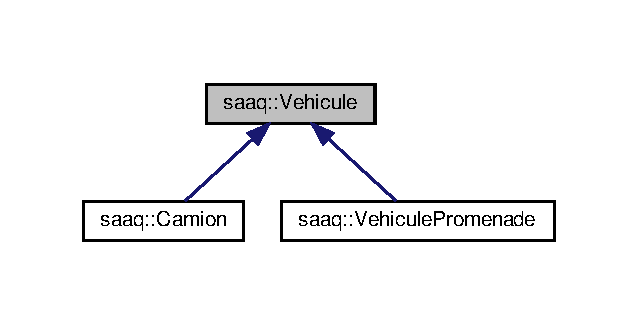
\includegraphics[width=306pt]{classsaaq_1_1Vehicule__inherit__graph}
\end{center}
\end{figure}
\subsection*{Public Member Functions}
\begin{DoxyCompactItemize}
\item 
\hyperlink{classsaaq_1_1Vehicule_a20f052188538616a6f54ee1061398319}{Vehicule} (const std\+::string \&p\+\_\+niv, const std\+::string \&p\+\_\+immatriculation, \hyperlink{classutil_1_1Date}{util\+::\+Date} \&p\+\_\+date\+Enregistrement)
\begin{DoxyCompactList}\small\item\em Constructeur d\textquotesingle{}un nouvel objet de la classe \hyperlink{classsaaq_1_1Vehicule}{Vehicule}. \end{DoxyCompactList}\item 
\mbox{\Hypertarget{classsaaq_1_1Vehicule_a24e65619f882d26dd3f2bfee25a7b3e6}\label{classsaaq_1_1Vehicule_a24e65619f882d26dd3f2bfee25a7b3e6}} 
virtual \hyperlink{classsaaq_1_1Vehicule}{Vehicule} $\ast$ {\bfseries clone} () const =0
\item 
virtual double \hyperlink{classsaaq_1_1Vehicule_a93570921069d25b6bc48cf04af176395}{tarification\+Annuelle} () const =0
\begin{DoxyCompactList}\small\item\em Retourne la tarification annuelle du vehicule. \end{DoxyCompactList}\item 
const std\+::string \& \hyperlink{classsaaq_1_1Vehicule_a8a7c31860afb58614a44ba89a9ddc224}{req\+Niv} () const
\begin{DoxyCompactList}\small\item\em Retourne le N\+IV. \end{DoxyCompactList}\item 
const std\+::string \& \hyperlink{classsaaq_1_1Vehicule_a2e8df437d34cc3b3e5008d5a5a819aae}{req\+Immatriculation} () const
\begin{DoxyCompactList}\small\item\em Retourne le numéro d\textquotesingle{}immatriculation. \end{DoxyCompactList}\item 
const \hyperlink{classutil_1_1Date}{util\+::\+Date} \hyperlink{classsaaq_1_1Vehicule_a650c5f764375e344e268391a5c3cf8b3}{req\+Date\+Enregistrement} () const
\begin{DoxyCompactList}\small\item\em Retourne la date d\textquotesingle{}enregistrement. \end{DoxyCompactList}\item 
virtual std\+::string \hyperlink{classsaaq_1_1Vehicule_a9d0ff95273ecd7858cf9bd12aac359ba}{req\+Vehicule\+Formate} () const
\begin{DoxyCompactList}\small\item\em Renvoie les informations de l\textquotesingle{}enregistrement dans un format console. \end{DoxyCompactList}\item 
bool \hyperlink{classsaaq_1_1Vehicule_a9dd4c5e7c74ebabd5f4ce651d21d79fc}{operator==} (const \hyperlink{classsaaq_1_1Vehicule}{Vehicule} \&p\+\_\+vehicule) const
\begin{DoxyCompactList}\small\item\em Surcharge de l\textquotesingle{}opérateur == qui permet de vérifier si la plaques et la date d\textquotesingle{}enregistrement sont identiques. \end{DoxyCompactList}\end{DoxyCompactItemize}
\subsection*{Protected Member Functions}
\begin{DoxyCompactItemize}
\item 
void \hyperlink{classsaaq_1_1Vehicule_a17c2ad3a6fabdf37c47811a9b0183e24}{asg\+Immatriculation} (const std\+::string \&p\+\_\+immatriculation)
\begin{DoxyCompactList}\small\item\em Assigne une nouvelle plaque automobile. \end{DoxyCompactList}\end{DoxyCompactItemize}


\subsection{Detailed Description}
Classe vehicule qui contient les informations d\textquotesingle{}une plaque automobile. Contient la plaque d\textquotesingle{}immatriculation, la date d\textquotesingle{}enregistrement et le N\+IV du vehicule. Des méthode qui permettent de nous donner chaques valeurs. Une méthode qui permet d\textquotesingle{}assigner une nouvelle plaque de vehicule. Une méthode qui permet d\textquotesingle{}afficher le tout dans un format console. 

\subsection{Constructor \& Destructor Documentation}
\mbox{\Hypertarget{classsaaq_1_1Vehicule_a20f052188538616a6f54ee1061398319}\label{classsaaq_1_1Vehicule_a20f052188538616a6f54ee1061398319}} 
\index{saaq\+::\+Vehicule@{saaq\+::\+Vehicule}!Vehicule@{Vehicule}}
\index{Vehicule@{Vehicule}!saaq\+::\+Vehicule@{saaq\+::\+Vehicule}}
\subsubsection{\texorpdfstring{Vehicule()}{Vehicule()}}
{\footnotesize\ttfamily saaq\+::\+Vehicule\+::\+Vehicule (\begin{DoxyParamCaption}\item[{const std\+::string \&}]{p\+\_\+niv,  }\item[{const std\+::string \&}]{p\+\_\+immatriculation,  }\item[{\hyperlink{classutil_1_1Date}{util\+::\+Date} \&}]{p\+\_\+date\+Enregistrement }\end{DoxyParamCaption})}



Constructeur d\textquotesingle{}un nouvel objet de la classe \hyperlink{classsaaq_1_1Vehicule}{Vehicule}. 


\begin{DoxyParams}[1]{Parameters}
\mbox{\tt in}  & {\em p\+\_\+niv} & N\+IV du vehicule \\
\hline
\mbox{\tt in}  & {\em p\+\_\+immatriculation} & immatriculation du vehicule \\
\hline
\mbox{\tt in}  & {\em p\+\_\+date\+Enregistrement} & date d\textquotesingle{}enregistrement \\
\hline
\end{DoxyParams}
\begin{DoxyPostcond}{Postcondition}
l\textquotesingle{}objet courant a été correctement créé et assigné 
\end{DoxyPostcond}
\begin{DoxyPrecond}{Precondition}
p\+\_\+niv, p\+\_\+immatriculation, p\+\_\+date\+Enregistrement sont valide 
\end{DoxyPrecond}
\begin{DoxyPostcond}{Postcondition}
m\+\_\+niv prend la valeur de p\+\_\+niv 

m\+\_\+immatriculation prend la valeur de p\+\_\+immatriculation 

m\+\_\+date\+Enregistrement prend la valeur de p\+\_\+date\+Enregistrement 
\end{DoxyPostcond}


\subsection{Member Function Documentation}
\mbox{\Hypertarget{classsaaq_1_1Vehicule_a17c2ad3a6fabdf37c47811a9b0183e24}\label{classsaaq_1_1Vehicule_a17c2ad3a6fabdf37c47811a9b0183e24}} 
\index{saaq\+::\+Vehicule@{saaq\+::\+Vehicule}!asg\+Immatriculation@{asg\+Immatriculation}}
\index{asg\+Immatriculation@{asg\+Immatriculation}!saaq\+::\+Vehicule@{saaq\+::\+Vehicule}}
\subsubsection{\texorpdfstring{asg\+Immatriculation()}{asgImmatriculation()}}
{\footnotesize\ttfamily void saaq\+::\+Vehicule\+::asg\+Immatriculation (\begin{DoxyParamCaption}\item[{const std\+::string \&}]{p\+\_\+immatriculation }\end{DoxyParamCaption})\hspace{0.3cm}{\ttfamily [protected]}}



Assigne une nouvelle plaque automobile. 


\begin{DoxyParams}[1]{Parameters}
\mbox{\tt in}  & {\em p\+\_\+immatriculation} & est la nouvelle plaque automobile qui est valide \\
\hline
\end{DoxyParams}
\begin{DoxyPrecond}{Precondition}
p\+\_\+immatriculation correspond a une plaque automobile valide 
\end{DoxyPrecond}
\begin{DoxyPostcond}{Postcondition}
m\+\_\+immatriculation prend la veleur de p\+\_\+immatriculation 
\end{DoxyPostcond}
\mbox{\Hypertarget{classsaaq_1_1Vehicule_a9dd4c5e7c74ebabd5f4ce651d21d79fc}\label{classsaaq_1_1Vehicule_a9dd4c5e7c74ebabd5f4ce651d21d79fc}} 
\index{saaq\+::\+Vehicule@{saaq\+::\+Vehicule}!operator==@{operator==}}
\index{operator==@{operator==}!saaq\+::\+Vehicule@{saaq\+::\+Vehicule}}
\subsubsection{\texorpdfstring{operator==()}{operator==()}}
{\footnotesize\ttfamily bool saaq\+::\+Vehicule\+::operator== (\begin{DoxyParamCaption}\item[{const \hyperlink{classsaaq_1_1Vehicule}{Vehicule} \&}]{p\+\_\+vehicule }\end{DoxyParamCaption}) const}



Surcharge de l\textquotesingle{}opérateur == qui permet de vérifier si la plaques et la date d\textquotesingle{}enregistrement sont identiques. 


\begin{DoxyParams}[1]{Parameters}
\mbox{\tt in}  & {\em p\+\_\+vehicule} & objet vehicule à comparer \\
\hline
\end{DoxyParams}
\begin{DoxyReturn}{Returns}
valeur booléene de la comparaison de la plaque et de la date d\textquotesingle{}enregistrement 
\end{DoxyReturn}
\mbox{\Hypertarget{classsaaq_1_1Vehicule_a650c5f764375e344e268391a5c3cf8b3}\label{classsaaq_1_1Vehicule_a650c5f764375e344e268391a5c3cf8b3}} 
\index{saaq\+::\+Vehicule@{saaq\+::\+Vehicule}!req\+Date\+Enregistrement@{req\+Date\+Enregistrement}}
\index{req\+Date\+Enregistrement@{req\+Date\+Enregistrement}!saaq\+::\+Vehicule@{saaq\+::\+Vehicule}}
\subsubsection{\texorpdfstring{req\+Date\+Enregistrement()}{reqDateEnregistrement()}}
{\footnotesize\ttfamily const \hyperlink{classutil_1_1Date}{util\+::\+Date} saaq\+::\+Vehicule\+::req\+Date\+Enregistrement (\begin{DoxyParamCaption}{ }\end{DoxyParamCaption}) const}



Retourne la date d\textquotesingle{}enregistrement. 

\begin{DoxyReturn}{Returns}
date d\textquotesingle{}enregistrement 
\end{DoxyReturn}
\mbox{\Hypertarget{classsaaq_1_1Vehicule_a2e8df437d34cc3b3e5008d5a5a819aae}\label{classsaaq_1_1Vehicule_a2e8df437d34cc3b3e5008d5a5a819aae}} 
\index{saaq\+::\+Vehicule@{saaq\+::\+Vehicule}!req\+Immatriculation@{req\+Immatriculation}}
\index{req\+Immatriculation@{req\+Immatriculation}!saaq\+::\+Vehicule@{saaq\+::\+Vehicule}}
\subsubsection{\texorpdfstring{req\+Immatriculation()}{reqImmatriculation()}}
{\footnotesize\ttfamily const std\+::string \& saaq\+::\+Vehicule\+::req\+Immatriculation (\begin{DoxyParamCaption}{ }\end{DoxyParamCaption}) const}



Retourne le numéro d\textquotesingle{}immatriculation. 

\begin{DoxyReturn}{Returns}
Le numéro d\textquotesingle{}immatriculation 
\end{DoxyReturn}
\mbox{\Hypertarget{classsaaq_1_1Vehicule_a8a7c31860afb58614a44ba89a9ddc224}\label{classsaaq_1_1Vehicule_a8a7c31860afb58614a44ba89a9ddc224}} 
\index{saaq\+::\+Vehicule@{saaq\+::\+Vehicule}!req\+Niv@{req\+Niv}}
\index{req\+Niv@{req\+Niv}!saaq\+::\+Vehicule@{saaq\+::\+Vehicule}}
\subsubsection{\texorpdfstring{req\+Niv()}{reqNiv()}}
{\footnotesize\ttfamily const std\+::string \& saaq\+::\+Vehicule\+::req\+Niv (\begin{DoxyParamCaption}{ }\end{DoxyParamCaption}) const}



Retourne le N\+IV. 

\begin{DoxyReturn}{Returns}
le N\+IV 
\end{DoxyReturn}
\mbox{\Hypertarget{classsaaq_1_1Vehicule_a9d0ff95273ecd7858cf9bd12aac359ba}\label{classsaaq_1_1Vehicule_a9d0ff95273ecd7858cf9bd12aac359ba}} 
\index{saaq\+::\+Vehicule@{saaq\+::\+Vehicule}!req\+Vehicule\+Formate@{req\+Vehicule\+Formate}}
\index{req\+Vehicule\+Formate@{req\+Vehicule\+Formate}!saaq\+::\+Vehicule@{saaq\+::\+Vehicule}}
\subsubsection{\texorpdfstring{req\+Vehicule\+Formate()}{reqVehiculeFormate()}}
{\footnotesize\ttfamily std\+::string saaq\+::\+Vehicule\+::req\+Vehicule\+Formate (\begin{DoxyParamCaption}{ }\end{DoxyParamCaption}) const\hspace{0.3cm}{\ttfamily [virtual]}}



Renvoie les informations de l\textquotesingle{}enregistrement dans un format console. 

\begin{DoxyReturn}{Returns}
Informations de la plaque automobile, son N\+IV et la date d\textquotesingle{}enregistrement 
\end{DoxyReturn}


Reimplemented in \hyperlink{classsaaq_1_1Camion_a7e352c9d011c145497fa19d16482bd9a}{saaq\+::\+Camion}, and \hyperlink{classsaaq_1_1VehiculePromenade_a338b22f240c47613ba08f37bf717658b}{saaq\+::\+Vehicule\+Promenade}.

\mbox{\Hypertarget{classsaaq_1_1Vehicule_a93570921069d25b6bc48cf04af176395}\label{classsaaq_1_1Vehicule_a93570921069d25b6bc48cf04af176395}} 
\index{saaq\+::\+Vehicule@{saaq\+::\+Vehicule}!tarification\+Annuelle@{tarification\+Annuelle}}
\index{tarification\+Annuelle@{tarification\+Annuelle}!saaq\+::\+Vehicule@{saaq\+::\+Vehicule}}
\subsubsection{\texorpdfstring{tarification\+Annuelle()}{tarificationAnnuelle()}}
{\footnotesize\ttfamily double saaq\+::\+Vehicule\+::tarification\+Annuelle (\begin{DoxyParamCaption}{ }\end{DoxyParamCaption}) const\hspace{0.3cm}{\ttfamily [pure virtual]}}



Retourne la tarification annuelle du vehicule. 

\begin{DoxyReturn}{Returns}
tarification annuelle 
\end{DoxyReturn}


Implemented in \hyperlink{classsaaq_1_1Camion_af01bdc48db3cdeb3bc29c8b864ffdad8}{saaq\+::\+Camion}, and \hyperlink{classsaaq_1_1VehiculePromenade_ad94d645be9862d1cd86953ca8a7777b9}{saaq\+::\+Vehicule\+Promenade}.



The documentation for this class was generated from the following files\+:\begin{DoxyCompactItemize}
\item 
\hyperlink{Vehicule_8h}{Vehicule.\+h}\item 
\hyperlink{Vehicule_8cpp}{Vehicule.\+cpp}\end{DoxyCompactItemize}

\hypertarget{classsaaq_1_1VehiculePromenade}{}\section{saaq\+:\+:Vehicule\+Promenade Class Reference}
\label{classsaaq_1_1VehiculePromenade}\index{saaq\+::\+Vehicule\+Promenade@{saaq\+::\+Vehicule\+Promenade}}


Classe \hyperlink{classsaaq_1_1VehiculePromenade}{Vehicule\+Promenade} qui contient les informations sur un \hyperlink{classsaaq_1_1Vehicule}{Vehicule} de Promenade Contient la plaque d\textquotesingle{}immatriculation, la date d\textquotesingle{}enregistrement, le nombre de place et le N\+IV du vehicule. Des méthode qui permettent de nous donner chaques valeurs. Une méthode qui permet d\textquotesingle{}assigner une nouvelle plaque de \hyperlink{classsaaq_1_1Vehicule}{Vehicule} de Promenade. Une méthode qui permet d\textquotesingle{}afficher le tout dans un format console.  




{\ttfamily \#include $<$Vehicule\+Promenade.\+h$>$}



Inheritance diagram for saaq\+:\+:Vehicule\+Promenade\+:\nopagebreak
\begin{figure}[H]
\begin{center}
\leavevmode
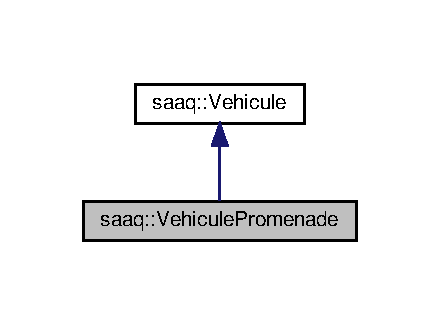
\includegraphics[width=211pt]{classsaaq_1_1VehiculePromenade__inherit__graph}
\end{center}
\end{figure}


Collaboration diagram for saaq\+:\+:Vehicule\+Promenade\+:\nopagebreak
\begin{figure}[H]
\begin{center}
\leavevmode
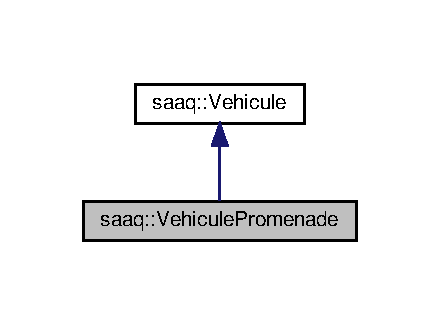
\includegraphics[width=211pt]{classsaaq_1_1VehiculePromenade__coll__graph}
\end{center}
\end{figure}
\subsection*{Public Member Functions}
\begin{DoxyCompactItemize}
\item 
\mbox{\Hypertarget{classsaaq_1_1VehiculePromenade_a5caaa3fa80ced57a49922fa44a127800}\label{classsaaq_1_1VehiculePromenade_a5caaa3fa80ced57a49922fa44a127800}} 
{\bfseries Vehicule\+Promenade} (const int p\+\_\+nb\+Places, const std\+::string \&p\+\_\+niv, const std\+::string p\+\_\+immatriculation, \hyperlink{classutil_1_1Date}{util\+::\+Date} \&p\+\_\+date\+Enregistrement)
\item 
const int \hyperlink{classsaaq_1_1VehiculePromenade_a71338b24fa5d12cc432b7f7d29917b75}{req\+\_\+nb\+Places} () const
\begin{DoxyCompactList}\small\item\em Retourne le nombre de place du vehicule de promenade. \end{DoxyCompactList}\item 
void \hyperlink{classsaaq_1_1VehiculePromenade_a86cbcf72ff776c5e79dcfd9703d7121e}{asg\+Immatriculation} (const std\+::string \&p\+\_\+immatriculation)
\begin{DoxyCompactList}\small\item\em Assigne une nouvelle plaque automobile de promenade. \end{DoxyCompactList}\item 
double \hyperlink{classsaaq_1_1VehiculePromenade_ad94d645be9862d1cd86953ca8a7777b9}{tarification\+Annuelle} () const
\begin{DoxyCompactList}\small\item\em Retourne la tarification Annuelle du vehicule de promenade. \end{DoxyCompactList}\item 
virtual \hyperlink{classsaaq_1_1Vehicule}{Vehicule} $\ast$ \hyperlink{classsaaq_1_1VehiculePromenade_ac4dc7715d78c2c0aca03c0eb5818bf4a}{clone} () const
\begin{DoxyCompactList}\small\item\em Retourne un clone de l\textquotesingle{}objet \hyperlink{classsaaq_1_1VehiculePromenade}{Vehicule\+Promenade}. \end{DoxyCompactList}\item 
virtual std\+::string \hyperlink{classsaaq_1_1VehiculePromenade_a338b22f240c47613ba08f37bf717658b}{req\+Vehicule\+Formate} () const
\begin{DoxyCompactList}\small\item\em Retourne une string contenant les informations contenues pour un \hyperlink{classsaaq_1_1Vehicule}{Vehicule} de Promenade. \end{DoxyCompactList}\end{DoxyCompactItemize}
\subsection*{Additional Inherited Members}


\subsection{Detailed Description}
Classe \hyperlink{classsaaq_1_1VehiculePromenade}{Vehicule\+Promenade} qui contient les informations sur un \hyperlink{classsaaq_1_1Vehicule}{Vehicule} de Promenade Contient la plaque d\textquotesingle{}immatriculation, la date d\textquotesingle{}enregistrement, le nombre de place et le N\+IV du vehicule. Des méthode qui permettent de nous donner chaques valeurs. Une méthode qui permet d\textquotesingle{}assigner une nouvelle plaque de \hyperlink{classsaaq_1_1Vehicule}{Vehicule} de Promenade. Une méthode qui permet d\textquotesingle{}afficher le tout dans un format console. 

\subsection{Member Function Documentation}
\mbox{\Hypertarget{classsaaq_1_1VehiculePromenade_a86cbcf72ff776c5e79dcfd9703d7121e}\label{classsaaq_1_1VehiculePromenade_a86cbcf72ff776c5e79dcfd9703d7121e}} 
\index{saaq\+::\+Vehicule\+Promenade@{saaq\+::\+Vehicule\+Promenade}!asg\+Immatriculation@{asg\+Immatriculation}}
\index{asg\+Immatriculation@{asg\+Immatriculation}!saaq\+::\+Vehicule\+Promenade@{saaq\+::\+Vehicule\+Promenade}}
\subsubsection{\texorpdfstring{asg\+Immatriculation()}{asgImmatriculation()}}
{\footnotesize\ttfamily void saaq\+::\+Vehicule\+Promenade\+::asg\+Immatriculation (\begin{DoxyParamCaption}\item[{const std\+::string \&}]{p\+\_\+immatriculation }\end{DoxyParamCaption})}



Assigne une nouvelle plaque automobile de promenade. 


\begin{DoxyParams}[1]{Parameters}
\mbox{\tt in}  & {\em p\+\_\+immatriculation} & est la nouvelle plaque automobile de promenade qui est valide \\
\hline
\end{DoxyParams}
\begin{DoxyPrecond}{Precondition}
p\+\_\+immatriculation correspond a une plaque automobile valide 
\end{DoxyPrecond}
\begin{DoxyPostcond}{Postcondition}
m\+\_\+immatriculation prend la veleur de p\+\_\+immatriculation 

p\+\_\+immatriculation est valide 
\end{DoxyPostcond}
\mbox{\Hypertarget{classsaaq_1_1VehiculePromenade_ac4dc7715d78c2c0aca03c0eb5818bf4a}\label{classsaaq_1_1VehiculePromenade_ac4dc7715d78c2c0aca03c0eb5818bf4a}} 
\index{saaq\+::\+Vehicule\+Promenade@{saaq\+::\+Vehicule\+Promenade}!clone@{clone}}
\index{clone@{clone}!saaq\+::\+Vehicule\+Promenade@{saaq\+::\+Vehicule\+Promenade}}
\subsubsection{\texorpdfstring{clone()}{clone()}}
{\footnotesize\ttfamily \hyperlink{classsaaq_1_1Vehicule}{Vehicule} $\ast$ saaq\+::\+Vehicule\+Promenade\+::clone (\begin{DoxyParamCaption}{ }\end{DoxyParamCaption}) const\hspace{0.3cm}{\ttfamily [virtual]}}



Retourne un clone de l\textquotesingle{}objet \hyperlink{classsaaq_1_1VehiculePromenade}{Vehicule\+Promenade}. 

\begin{DoxyReturn}{Returns}
une copie de \hyperlink{classsaaq_1_1VehiculePromenade}{Vehicule\+Promenade} 
\end{DoxyReturn}


Implements \hyperlink{classsaaq_1_1Vehicule}{saaq\+::\+Vehicule}.

\mbox{\Hypertarget{classsaaq_1_1VehiculePromenade_a71338b24fa5d12cc432b7f7d29917b75}\label{classsaaq_1_1VehiculePromenade_a71338b24fa5d12cc432b7f7d29917b75}} 
\index{saaq\+::\+Vehicule\+Promenade@{saaq\+::\+Vehicule\+Promenade}!req\+\_\+nb\+Places@{req\+\_\+nb\+Places}}
\index{req\+\_\+nb\+Places@{req\+\_\+nb\+Places}!saaq\+::\+Vehicule\+Promenade@{saaq\+::\+Vehicule\+Promenade}}
\subsubsection{\texorpdfstring{req\+\_\+nb\+Places()}{req\_nbPlaces()}}
{\footnotesize\ttfamily const int saaq\+::\+Vehicule\+Promenade\+::req\+\_\+nb\+Places (\begin{DoxyParamCaption}{ }\end{DoxyParamCaption}) const}



Retourne le nombre de place du vehicule de promenade. 

\begin{DoxyReturn}{Returns}
le nombre de place du vehicule de promenade 
\end{DoxyReturn}
\mbox{\Hypertarget{classsaaq_1_1VehiculePromenade_a338b22f240c47613ba08f37bf717658b}\label{classsaaq_1_1VehiculePromenade_a338b22f240c47613ba08f37bf717658b}} 
\index{saaq\+::\+Vehicule\+Promenade@{saaq\+::\+Vehicule\+Promenade}!req\+Vehicule\+Formate@{req\+Vehicule\+Formate}}
\index{req\+Vehicule\+Formate@{req\+Vehicule\+Formate}!saaq\+::\+Vehicule\+Promenade@{saaq\+::\+Vehicule\+Promenade}}
\subsubsection{\texorpdfstring{req\+Vehicule\+Formate()}{reqVehiculeFormate()}}
{\footnotesize\ttfamily std\+::string saaq\+::\+Vehicule\+Promenade\+::req\+Vehicule\+Formate (\begin{DoxyParamCaption}{ }\end{DoxyParamCaption}) const\hspace{0.3cm}{\ttfamily [virtual]}}



Retourne une string contenant les informations contenues pour un \hyperlink{classsaaq_1_1Vehicule}{Vehicule} de Promenade. 

\begin{DoxyReturn}{Returns}
informations de \hyperlink{classsaaq_1_1VehiculePromenade}{Vehicule\+Promenade} 
\end{DoxyReturn}


Reimplemented from \hyperlink{classsaaq_1_1Vehicule_a9d0ff95273ecd7858cf9bd12aac359ba}{saaq\+::\+Vehicule}.

\mbox{\Hypertarget{classsaaq_1_1VehiculePromenade_ad94d645be9862d1cd86953ca8a7777b9}\label{classsaaq_1_1VehiculePromenade_ad94d645be9862d1cd86953ca8a7777b9}} 
\index{saaq\+::\+Vehicule\+Promenade@{saaq\+::\+Vehicule\+Promenade}!tarification\+Annuelle@{tarification\+Annuelle}}
\index{tarification\+Annuelle@{tarification\+Annuelle}!saaq\+::\+Vehicule\+Promenade@{saaq\+::\+Vehicule\+Promenade}}
\subsubsection{\texorpdfstring{tarification\+Annuelle()}{tarificationAnnuelle()}}
{\footnotesize\ttfamily double saaq\+::\+Vehicule\+Promenade\+::tarification\+Annuelle (\begin{DoxyParamCaption}{ }\end{DoxyParamCaption}) const\hspace{0.3cm}{\ttfamily [virtual]}}



Retourne la tarification Annuelle du vehicule de promenade. 

\begin{DoxyReturn}{Returns}
la tarification Annuelle du vehicule de promenade 
\end{DoxyReturn}


Implements \hyperlink{classsaaq_1_1Vehicule_a93570921069d25b6bc48cf04af176395}{saaq\+::\+Vehicule}.



The documentation for this class was generated from the following files\+:\begin{DoxyCompactItemize}
\item 
\hyperlink{VehiculePromenade_8h}{Vehicule\+Promenade.\+h}\item 
\hyperlink{VehiculePromenade_8cpp}{Vehicule\+Promenade.\+cpp}\end{DoxyCompactItemize}

\chapter{File Documentation}
\hypertarget{Camion_8cpp}{}\section{Camion.\+cpp File Reference}
\label{Camion_8cpp}\index{Camion.\+cpp@{Camion.\+cpp}}


Fichier d\textquotesingle{}implémentation de la classe Camion.  


{\ttfamily \#include \char`\"{}Camion.\+h\char`\"{}}\newline
{\ttfamily \#include \char`\"{}Vehicule.\+h\char`\"{}}\newline
{\ttfamily \#include \char`\"{}Date.\+h\char`\"{}}\newline
{\ttfamily \#include $<$iostream$>$}\newline
{\ttfamily \#include $<$string$>$}\newline
{\ttfamily \#include $<$sstream$>$}\newline
Include dependency graph for Camion.\+cpp\+:\nopagebreak
\begin{figure}[H]
\begin{center}
\leavevmode
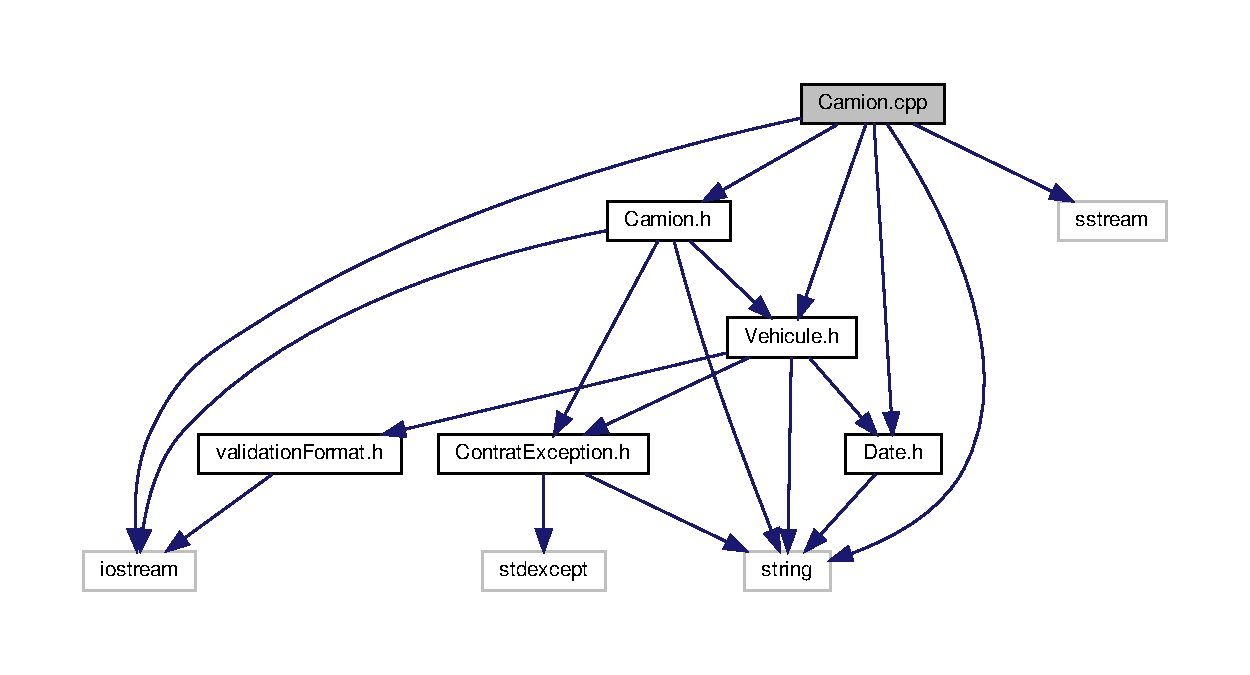
\includegraphics[width=350pt]{Camion_8cpp__incl}
\end{center}
\end{figure}


\subsection{Detailed Description}
Fichier d\textquotesingle{}implémentation de la classe Camion. 

\begin{DoxyDate}{Date}
2019-\/10-\/15 
\end{DoxyDate}
\begin{DoxyAuthor}{Author}
Renaud Morin 
\end{DoxyAuthor}

\hypertarget{Camion_8h}{}\section{Camion.\+h File Reference}
\label{Camion_8h}\index{Camion.\+h@{Camion.\+h}}


Fichier déclaration de la classe Camion.  


{\ttfamily \#include $<$string$>$}\newline
{\ttfamily \#include \char`\"{}Vehicule.\+h\char`\"{}}\newline
{\ttfamily \#include $<$iostream$>$}\newline
{\ttfamily \#include \char`\"{}Contrat\+Exception.\+h\char`\"{}}\newline
Include dependency graph for Camion.\+h\+:\nopagebreak
\begin{figure}[H]
\begin{center}
\leavevmode
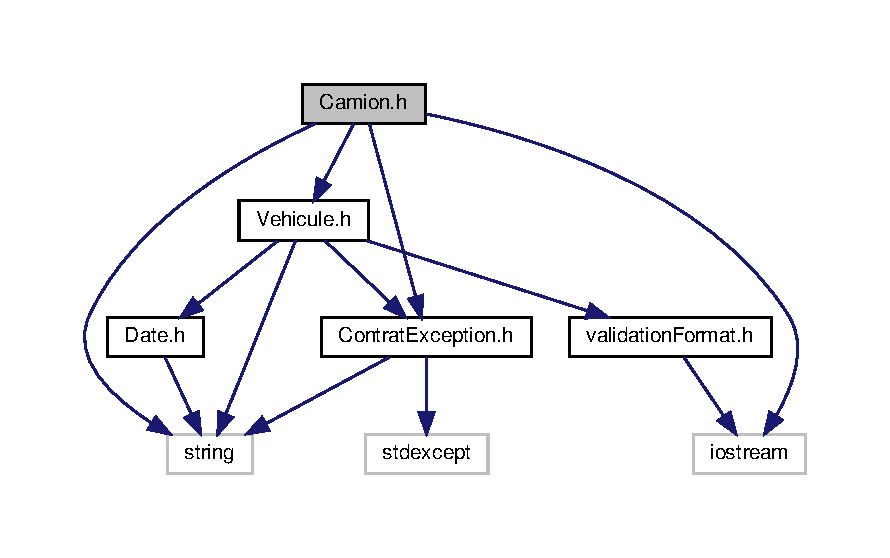
\includegraphics[width=350pt]{Camion_8h__incl}
\end{center}
\end{figure}
This graph shows which files directly or indirectly include this file\+:\nopagebreak
\begin{figure}[H]
\begin{center}
\leavevmode
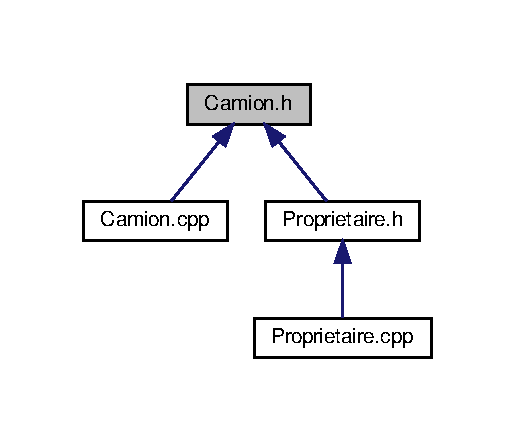
\includegraphics[width=247pt]{Camion_8h__dep__incl}
\end{center}
\end{figure}
\subsection*{Classes}
\begin{DoxyCompactItemize}
\item 
class \hyperlink{classsaaq_1_1Camion}{saaq\+::\+Camion}
\begin{DoxyCompactList}\small\item\em Classe \hyperlink{classsaaq_1_1Camion}{Camion} qui contient les informations sur un \hyperlink{classsaaq_1_1Camion}{Camion} Contient la plaque d\textquotesingle{}immatriculation, la date d\textquotesingle{}enregistrement, le poid, le nombre d\textquotesingle{}essieu et le N\+IV du camion. Des méthode qui permettent de nous donner chaques valeurs. Une méthode qui permet d\textquotesingle{}assigner une nouvelle plaque de camion. Une méthode qui permet d\textquotesingle{}afficher le tout dans un format console. \end{DoxyCompactList}\end{DoxyCompactItemize}


\subsection{Detailed Description}
Fichier déclaration de la classe Camion. 

\begin{DoxyDate}{Date}
2019-\/10-\/15 
\end{DoxyDate}
\begin{DoxyAuthor}{Author}
Renaud Morin 
\end{DoxyAuthor}

\hypertarget{ContratException_8cpp}{}\section{Contrat\+Exception.\+cpp File Reference}
\label{ContratException_8cpp}\index{Contrat\+Exception.\+cpp@{Contrat\+Exception.\+cpp}}


Implantation de la classe \hyperlink{classContratException}{Contrat\+Exception} et de ses héritiers.  


{\ttfamily \#include \char`\"{}Contrat\+Exception.\+h\char`\"{}}\newline
{\ttfamily \#include $<$sstream$>$}\newline
Include dependency graph for Contrat\+Exception.\+cpp\+:\nopagebreak
\begin{figure}[H]
\begin{center}
\leavevmode
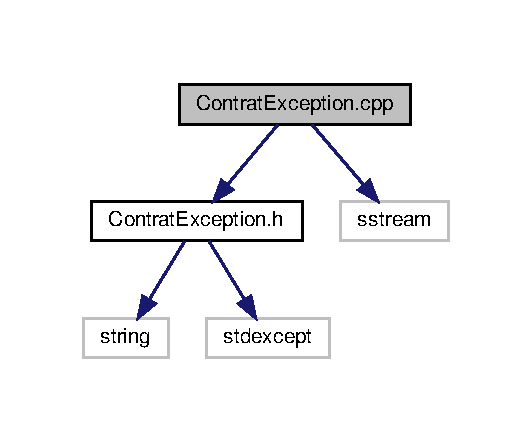
\includegraphics[width=255pt]{ContratException_8cpp__incl}
\end{center}
\end{figure}


\subsection{Detailed Description}
Implantation de la classe \hyperlink{classContratException}{Contrat\+Exception} et de ses héritiers. 

\begin{DoxyAuthor}{Author}
administrateur 
\end{DoxyAuthor}

\hypertarget{ContratException_8h}{}\section{Contrat\+Exception.\+h File Reference}
\label{ContratException_8h}\index{Contrat\+Exception.\+h@{Contrat\+Exception.\+h}}


Fichier contenant la déclaration de la classe \hyperlink{classContratException}{Contrat\+Exception} et de ses héritiers.  


{\ttfamily \#include $<$string$>$}\newline
{\ttfamily \#include $<$stdexcept$>$}\newline
Include dependency graph for Contrat\+Exception.\+h\+:\nopagebreak
\begin{figure}[H]
\begin{center}
\leavevmode
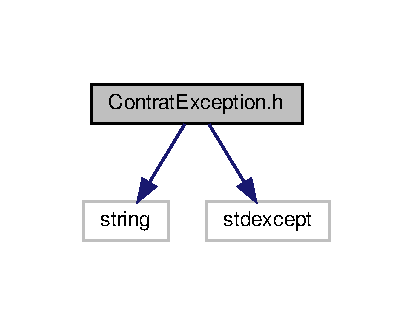
\includegraphics[width=198pt]{ContratException_8h__incl}
\end{center}
\end{figure}
This graph shows which files directly or indirectly include this file\+:\nopagebreak
\begin{figure}[H]
\begin{center}
\leavevmode
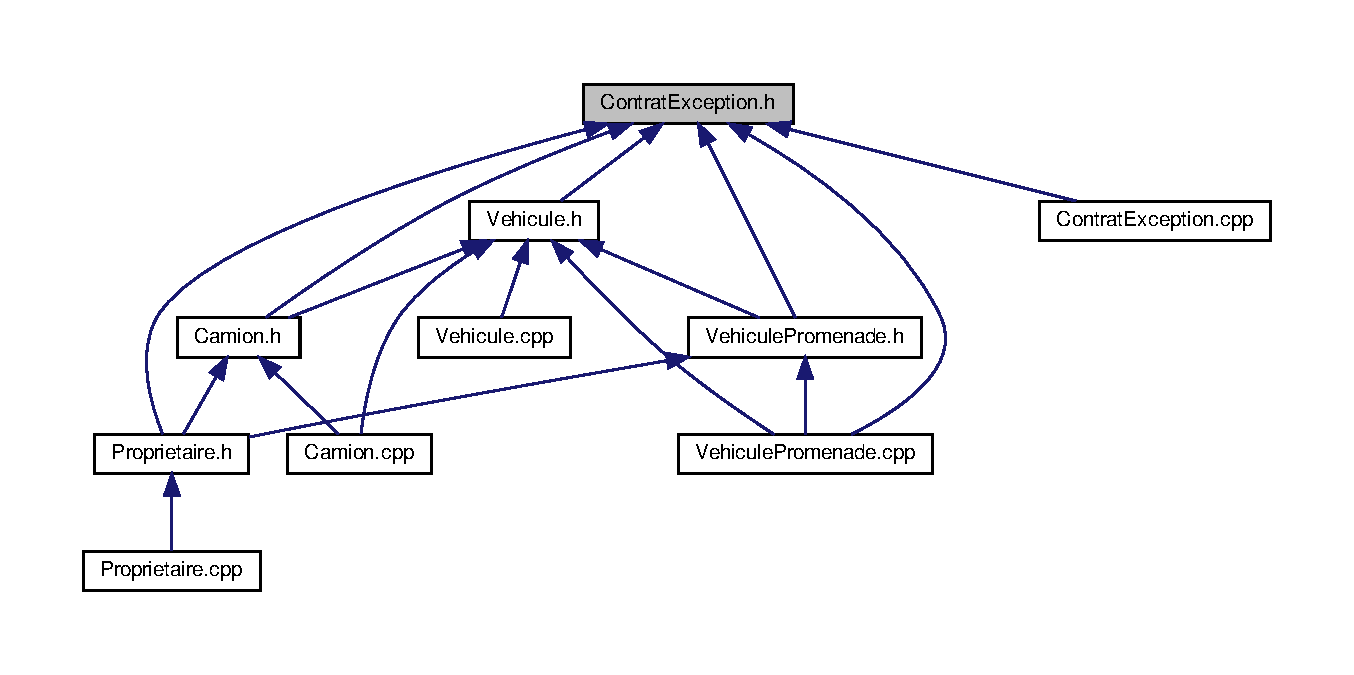
\includegraphics[width=350pt]{ContratException_8h__dep__incl}
\end{center}
\end{figure}
\subsection*{Classes}
\begin{DoxyCompactItemize}
\item 
class \hyperlink{classContratException}{Contrat\+Exception}
\begin{DoxyCompactList}\small\item\em Classe de base des exceptions de contrat. \end{DoxyCompactList}\item 
class \hyperlink{classAssertionException}{Assertion\+Exception}
\begin{DoxyCompactList}\small\item\em Classe pour la gestion des erreurs d\textquotesingle{}assertion. \end{DoxyCompactList}\item 
class \hyperlink{classPreconditionException}{Precondition\+Exception}
\begin{DoxyCompactList}\small\item\em Classe pour la gestion des erreurs de précondition. \end{DoxyCompactList}\item 
class \hyperlink{classPostconditionException}{Postcondition\+Exception}
\begin{DoxyCompactList}\small\item\em Classe pour la gestion des erreurs de postcondition. \end{DoxyCompactList}\item 
class \hyperlink{classInvariantException}{Invariant\+Exception}
\begin{DoxyCompactList}\small\item\em Classe pour la gestion des erreurs d\textquotesingle{}invariant. \end{DoxyCompactList}\end{DoxyCompactItemize}
\subsection*{Macros}
\begin{DoxyCompactItemize}
\item 
\mbox{\Hypertarget{ContratException_8h_a52dddc2c198c58b53b201c313934e40c}\label{ContratException_8h_a52dddc2c198c58b53b201c313934e40c}} 
\#define {\bfseries I\+N\+V\+A\+R\+I\+A\+N\+TS}()~verifie\+Invariant()
\item 
\mbox{\Hypertarget{ContratException_8h_abe6e3e0ff48f8595570e6485b506a8c4}\label{ContratException_8h_abe6e3e0ff48f8595570e6485b506a8c4}} 
\#define {\bfseries A\+S\+S\+E\+R\+T\+I\+ON}(f)~if (!(f)) throw \hyperlink{classAssertionException}{Assertion\+Exception}(\+\_\+\+\_\+\+F\+I\+L\+E\+\_\+\+\_\+,\+\_\+\+\_\+\+L\+I\+N\+E\+\_\+\+\_\+, \#f);
\item 
\mbox{\Hypertarget{ContratException_8h_acb3361bd87fc697a57b7286a9998c106}\label{ContratException_8h_acb3361bd87fc697a57b7286a9998c106}} 
\#define {\bfseries P\+R\+E\+C\+O\+N\+D\+I\+T\+I\+ON}(f)~if (!(f)) throw \hyperlink{classPreconditionException}{Precondition\+Exception}(\+\_\+\+\_\+\+F\+I\+L\+E\+\_\+\+\_\+, \+\_\+\+\_\+\+L\+I\+N\+E\+\_\+\+\_\+, \#f);
\item 
\mbox{\Hypertarget{ContratException_8h_a438b75c0c77a1ce8d1e914f9f04ea548}\label{ContratException_8h_a438b75c0c77a1ce8d1e914f9f04ea548}} 
\#define {\bfseries P\+O\+S\+T\+C\+O\+N\+D\+I\+T\+I\+ON}(f)~if (!(f)) throw \hyperlink{classPostconditionException}{Postcondition\+Exception}(\+\_\+\+\_\+\+F\+I\+L\+E\+\_\+\+\_\+, \+\_\+\+\_\+\+L\+I\+N\+E\+\_\+\+\_\+, \#f);
\item 
\mbox{\Hypertarget{ContratException_8h_a08f80155f47e05681c2b9bb9c5f6fffe}\label{ContratException_8h_a08f80155f47e05681c2b9bb9c5f6fffe}} 
\#define {\bfseries I\+N\+V\+A\+R\+I\+A\+NT}(f)~if (!(f)) throw \hyperlink{classInvariantException}{Invariant\+Exception}(\+\_\+\+\_\+\+F\+I\+L\+E\+\_\+\+\_\+,\+\_\+\+\_\+\+L\+I\+N\+E\+\_\+\+\_\+, \#f);
\end{DoxyCompactItemize}


\subsection{Detailed Description}
Fichier contenant la déclaration de la classe \hyperlink{classContratException}{Contrat\+Exception} et de ses héritiers. 

\begin{DoxyAuthor}{Author}
administrateur 
\end{DoxyAuthor}

\hypertarget{Date_8cpp}{}\section{Date.\+cpp File Reference}
\label{Date_8cpp}\index{Date.\+cpp@{Date.\+cpp}}


Implantation de la classe Date.  


{\ttfamily \#include \char`\"{}Date.\+h\char`\"{}}\newline
{\ttfamily \#include $<$sstream$>$}\newline
{\ttfamily \#include $<$ctime$>$}\newline
Include dependency graph for Date.\+cpp\+:\nopagebreak
\begin{figure}[H]
\begin{center}
\leavevmode
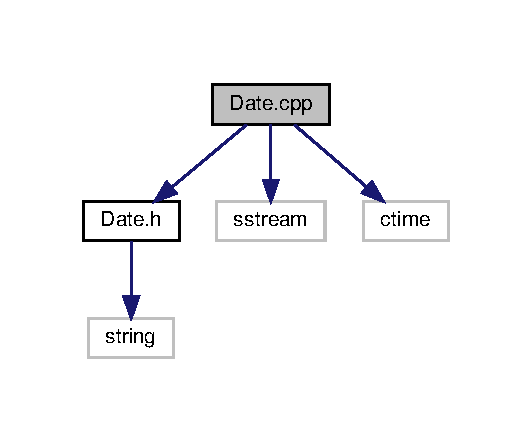
\includegraphics[width=255pt]{Date_8cpp__incl}
\end{center}
\end{figure}
\subsection*{Functions}
\begin{DoxyCompactItemize}
\item 
ostream \& \hyperlink{Date_8cpp_a795c6fa40e8fbe7cf36a4dd3413b93ae}{util\+::operator$<$$<$} (ostream \&p\+\_\+os, const Date \&p\+\_\+date)
\begin{DoxyCompactList}\small\item\em surcharge de la fonction $<$$<$ d\textquotesingle{}écriture dans une ostream \end{DoxyCompactList}\end{DoxyCompactItemize}


\subsection{Detailed Description}
Implantation de la classe Date. 

\begin{DoxyAuthor}{Author}
Yves Roy Version initiale, T\+HE 
\end{DoxyAuthor}
\begin{DoxyVersion}{Version}
3.\+3 sans contrat 
\end{DoxyVersion}


\subsection{Function Documentation}
\mbox{\Hypertarget{Date_8cpp_file_a795c6fa40e8fbe7cf36a4dd3413b93ae}\label{Date_8cpp_file_a795c6fa40e8fbe7cf36a4dd3413b93ae}} 
\index{Date.\+cpp@{Date.\+cpp}!operator$<$$<$@{operator$<$$<$}}
\index{operator$<$$<$@{operator$<$$<$}!Date.\+cpp@{Date.\+cpp}}
\subsubsection{\texorpdfstring{operator$<$$<$()}{operator<<()}}
{\footnotesize\ttfamily ostream\& util\+::operator$<$$<$ (\begin{DoxyParamCaption}\item[{ostream \&}]{p\+\_\+os,  }\item[{const \hyperlink{classutil_1_1Date}{Date} \&}]{p\+\_\+date }\end{DoxyParamCaption})}



surcharge de la fonction $<$$<$ d\textquotesingle{}écriture dans une ostream 


\begin{DoxyParams}[1]{Parameters}
\mbox{\tt in}  & {\em p\+\_\+os} & une stream vide dans laquelle on va écrire \\
\hline
\mbox{\tt in}  & {\em p\+\_\+date} & qui est une date valide \\
\hline
\end{DoxyParams}
\begin{DoxyReturn}{Returns}
la stream dans laquelle on a écrit la date 
\end{DoxyReturn}

\hypertarget{Date_8h}{}\section{Date.\+h File Reference}
\label{Date_8h}\index{Date.\+h@{Date.\+h}}


Fichier qui contient l\textquotesingle{}interface de la classe Date qui sert au maintien et à la manipulation des dates.  


{\ttfamily \#include $<$string$>$}\newline
Include dependency graph for Date.\+h\+:\nopagebreak
\begin{figure}[H]
\begin{center}
\leavevmode
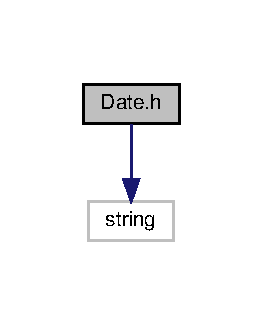
\includegraphics[width=126pt]{Date_8h__incl}
\end{center}
\end{figure}
This graph shows which files directly or indirectly include this file\+:\nopagebreak
\begin{figure}[H]
\begin{center}
\leavevmode
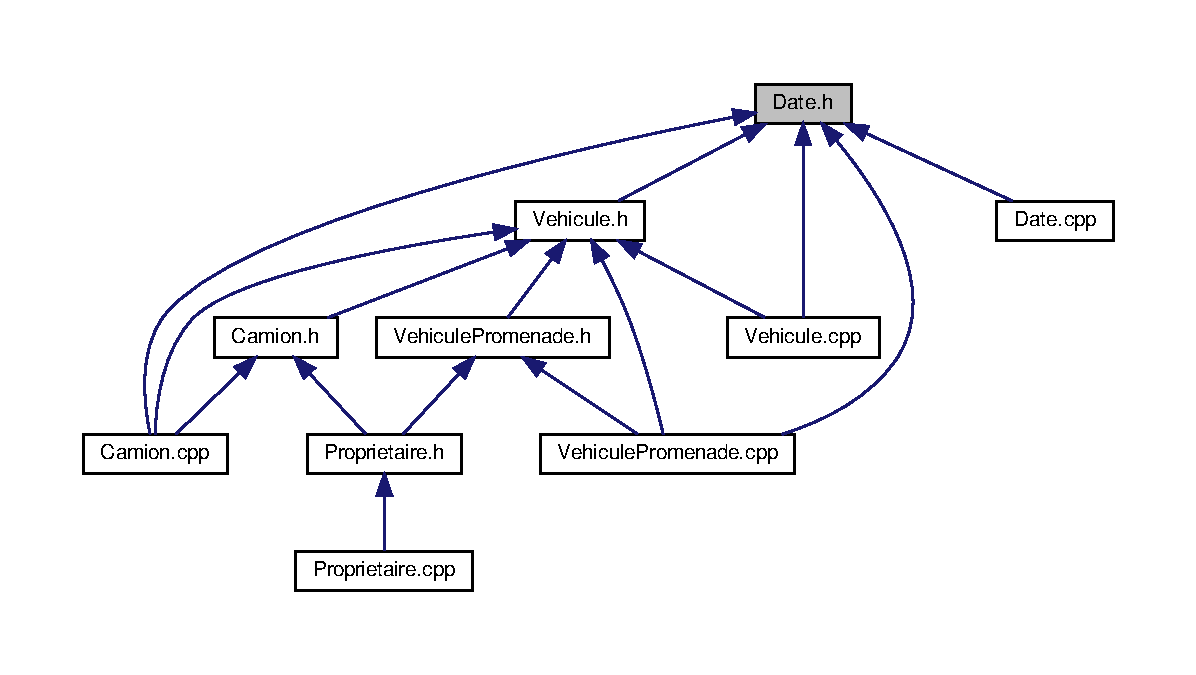
\includegraphics[width=350pt]{Date_8h__dep__incl}
\end{center}
\end{figure}
\subsection*{Classes}
\begin{DoxyCompactItemize}
\item 
class \hyperlink{classutil_1_1Date}{util\+::\+Date}
\begin{DoxyCompactList}\small\item\em Cette classe sert au maintien et à la manipulation des dates. \end{DoxyCompactList}\end{DoxyCompactItemize}


\subsection{Detailed Description}
Fichier qui contient l\textquotesingle{}interface de la classe Date qui sert au maintien et à la manipulation des dates. 

\begin{DoxyAuthor}{Author}
Yves Roy Version initiale, T\+HE 
\end{DoxyAuthor}
\begin{DoxyVersion}{Version}
3.\+2 sans contrat 
\end{DoxyVersion}

\hypertarget{Proprietaire_8cpp}{}\section{Proprietaire.\+cpp File Reference}
\label{Proprietaire_8cpp}\index{Proprietaire.\+cpp@{Proprietaire.\+cpp}}


Fichier d\textquotesingle{}implémentation de la classe Proprietaire.  


{\ttfamily \#include \char`\"{}Proprietaire.\+h\char`\"{}}\newline
{\ttfamily \#include $<$iostream$>$}\newline
{\ttfamily \#include $<$sstream$>$}\newline
{\ttfamily \#include $<$string$>$}\newline
Include dependency graph for Proprietaire.\+cpp\+:\nopagebreak
\begin{figure}[H]
\begin{center}
\leavevmode
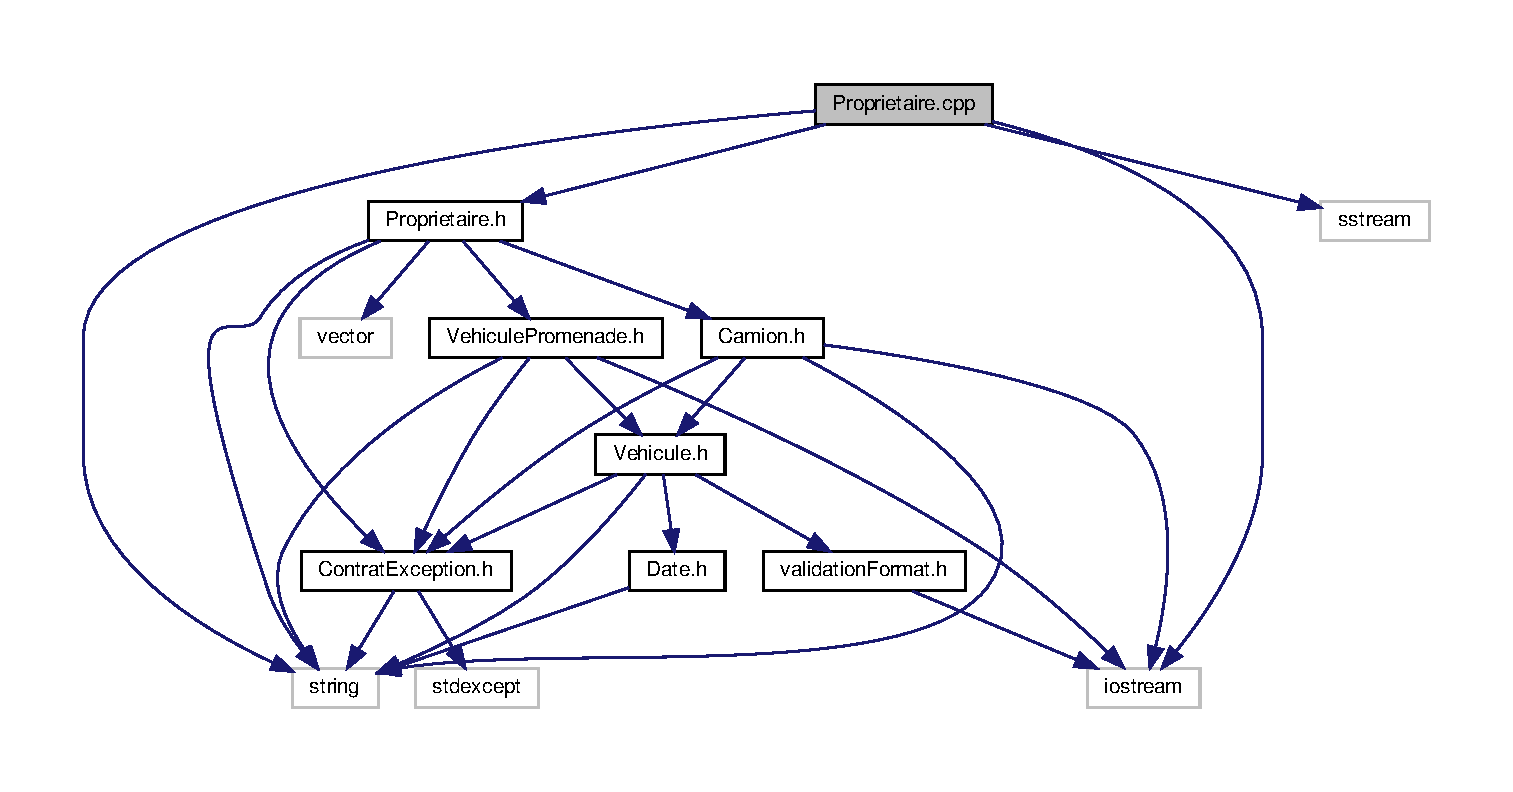
\includegraphics[width=350pt]{Proprietaire_8cpp__incl}
\end{center}
\end{figure}


\subsection{Detailed Description}
Fichier d\textquotesingle{}implémentation de la classe Proprietaire. 

\begin{DoxyDate}{Date}
2019-\/10-\/15 
\end{DoxyDate}
\begin{DoxyAuthor}{Author}
Renaud Morin 
\end{DoxyAuthor}

\hypertarget{Proprietaire_8h}{}\section{Proprietaire.\+h File Reference}
\label{Proprietaire_8h}\index{Proprietaire.\+h@{Proprietaire.\+h}}


Fichier declaration de la classe Proprietaire.  


{\ttfamily \#include $<$string$>$}\newline
{\ttfamily \#include \char`\"{}Camion.\+h\char`\"{}}\newline
{\ttfamily \#include \char`\"{}Vehicule\+Promenade.\+h\char`\"{}}\newline
{\ttfamily \#include \char`\"{}Contrat\+Exception.\+h\char`\"{}}\newline
{\ttfamily \#include $<$vector$>$}\newline
Include dependency graph for Proprietaire.\+h\+:\nopagebreak
\begin{figure}[H]
\begin{center}
\leavevmode
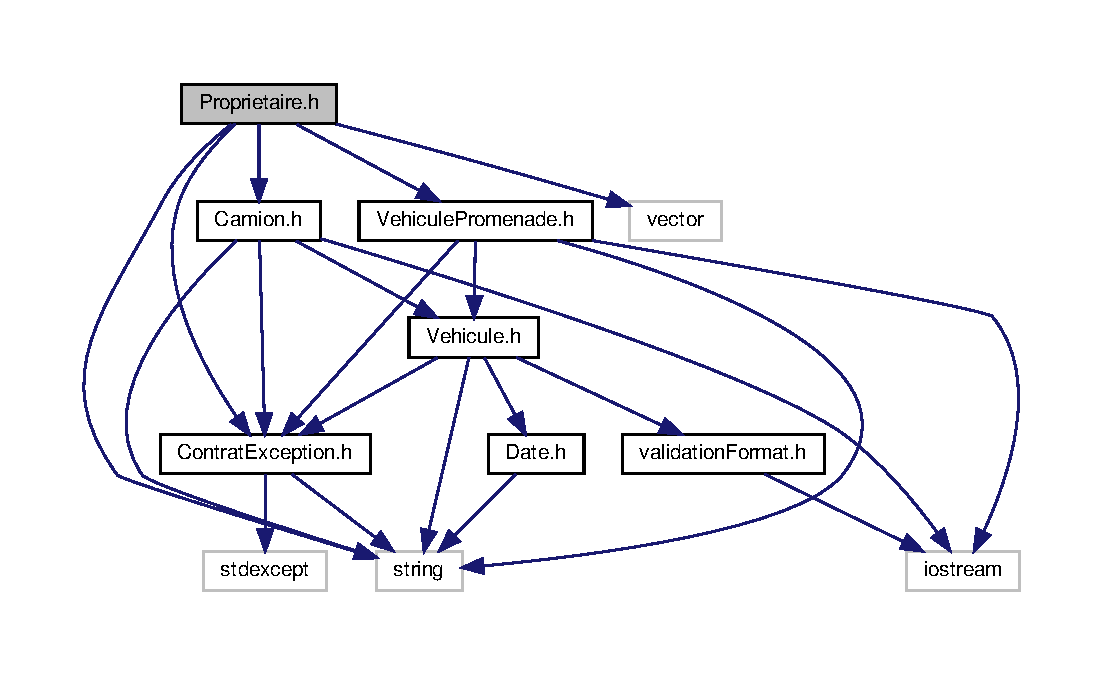
\includegraphics[width=350pt]{Proprietaire_8h__incl}
\end{center}
\end{figure}
This graph shows which files directly or indirectly include this file\+:\nopagebreak
\begin{figure}[H]
\begin{center}
\leavevmode
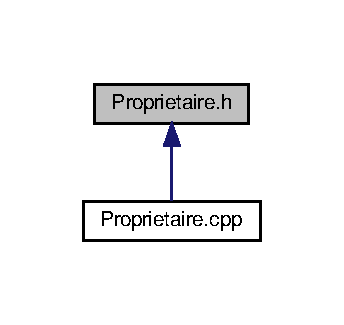
\includegraphics[width=165pt]{Proprietaire_8h__dep__incl}
\end{center}
\end{figure}
\subsection*{Classes}
\begin{DoxyCompactItemize}
\item 
class \hyperlink{classsaaq_1_1Proprietaire}{saaq\+::\+Proprietaire}
\begin{DoxyCompactList}\small\item\em Classe \hyperlink{classsaaq_1_1Proprietaire}{Proprietaire} qui contient les Camions et \hyperlink{classsaaq_1_1Vehicule}{Vehicule} de promenade -\/\+Accesseurs pour tous ses attributs -\/\+Assigner une nouvelle plaque automobile -\/\+Une methode qui retourne le tout de facon formate. \end{DoxyCompactList}\end{DoxyCompactItemize}


\subsection{Detailed Description}
Fichier declaration de la classe Proprietaire. 

\begin{DoxyDate}{Date}
2019-\/10-\/15 
\end{DoxyDate}
\begin{DoxyAuthor}{Author}
Renaud Morin 
\end{DoxyAuthor}

\hypertarget{validationFormat_8cpp}{}\section{validation\+Format.\+cpp File Reference}
\label{validationFormat_8cpp}\index{validation\+Format.\+cpp@{validation\+Format.\+cpp}}


Fichier permettant de valider une plaque automobile et un N\+IV.  


{\ttfamily \#include $<$iostream$>$}\newline
Include dependency graph for validation\+Format.\+cpp\+:\nopagebreak
\begin{figure}[H]
\begin{center}
\leavevmode
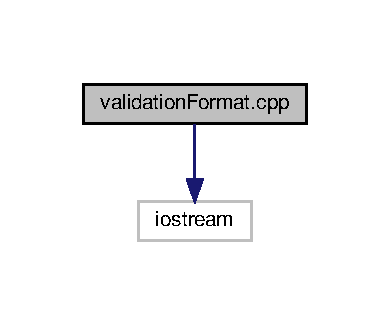
\includegraphics[width=187pt]{validationFormat_8cpp__incl}
\end{center}
\end{figure}
\subsection*{Functions}
\begin{DoxyCompactItemize}
\item 
bool \hyperlink{validationFormat_8cpp_a54e96460aa1c34b195351e8bb3cffeef}{util\+::valider\+Immatriculation} (const std\+::string \&p\+\_\+immatriculation)
\begin{DoxyCompactList}\small\item\em Fonction qui permet de valider le format dune plaque dimmatriculation. \end{DoxyCompactList}\item 
bool \hyperlink{validationFormat_8cpp_a7d9e1cb34ea051b7bb3203e0045ae3a3}{util\+::valider\+Niv} (const std\+::string \&p\+\_\+niv)
\begin{DoxyCompactList}\small\item\em Fonction qui permet de valider le format dun N\+IV. \end{DoxyCompactList}\item 
bool \hyperlink{validationFormat_8cpp_a4cf20d6bfbd40c3a521faafe28f1edde}{util\+::valider\+Immatriculation\+Camion} (const std\+::string \&p\+\_\+immatriculation)
\begin{DoxyCompactList}\small\item\em Fonction qui permet de valider le format dune plaque d\textquotesingle{}immatriculation de camion. \end{DoxyCompactList}\item 
bool \hyperlink{validationFormat_8cpp_a7bdc44b565fc0da4d7244670d00ce416}{util\+::valider\+Immatriculation\+Promenade} (const std\+::string \&p\+\_\+immatriculation)
\begin{DoxyCompactList}\small\item\em Fonction qui permet de valider le format dune plaque d\textquotesingle{}immatriculation de promenade. \end{DoxyCompactList}\end{DoxyCompactItemize}


\subsection{Detailed Description}
Fichier permettant de valider une plaque automobile et un N\+IV. 

\begin{DoxyDate}{Date}
2019-\/10-\/15 
\end{DoxyDate}
\begin{DoxyAuthor}{Author}
Renaud Morin 
\end{DoxyAuthor}


\subsection{Function Documentation}
\mbox{\Hypertarget{validationFormat_8cpp_file_a54e96460aa1c34b195351e8bb3cffeef}\label{validationFormat_8cpp_file_a54e96460aa1c34b195351e8bb3cffeef}} 
\index{validation\+Format.\+cpp@{validation\+Format.\+cpp}!valider\+Immatriculation@{valider\+Immatriculation}}
\index{valider\+Immatriculation@{valider\+Immatriculation}!validation\+Format.\+cpp@{validation\+Format.\+cpp}}
\subsubsection{\texorpdfstring{valider\+Immatriculation()}{validerImmatriculation()}}
{\footnotesize\ttfamily bool util\+::valider\+Immatriculation (\begin{DoxyParamCaption}\item[{const std\+::string \&}]{p\+\_\+immatriculation }\end{DoxyParamCaption})}



Fonction qui permet de valider le format dune plaque dimmatriculation. 


\begin{DoxyParams}[1]{Parameters}
\mbox{\tt in}  & {\em p\+\_\+immatriculation} & numero de plaque a verifier \\
\hline
\end{DoxyParams}
\begin{DoxyReturn}{Returns}
valeur booléenne selon la validité de la plaque automobile 
\end{DoxyReturn}
\mbox{\Hypertarget{validationFormat_8cpp_file_a4cf20d6bfbd40c3a521faafe28f1edde}\label{validationFormat_8cpp_file_a4cf20d6bfbd40c3a521faafe28f1edde}} 
\index{validation\+Format.\+cpp@{validation\+Format.\+cpp}!valider\+Immatriculation\+Camion@{valider\+Immatriculation\+Camion}}
\index{valider\+Immatriculation\+Camion@{valider\+Immatriculation\+Camion}!validation\+Format.\+cpp@{validation\+Format.\+cpp}}
\subsubsection{\texorpdfstring{valider\+Immatriculation\+Camion()}{validerImmatriculationCamion()}}
{\footnotesize\ttfamily bool util\+::valider\+Immatriculation\+Camion (\begin{DoxyParamCaption}\item[{const std\+::string \&}]{p\+\_\+immatriculation }\end{DoxyParamCaption})}



Fonction qui permet de valider le format dune plaque d\textquotesingle{}immatriculation de camion. 


\begin{DoxyParams}[1]{Parameters}
\mbox{\tt in}  & {\em p\+\_\+immatriculation} & numero de plaque a verifier \\
\hline
\end{DoxyParams}
\begin{DoxyReturn}{Returns}
valeur booléenne selon la validité de la plaque de camion 
\end{DoxyReturn}
\mbox{\Hypertarget{validationFormat_8cpp_file_a7bdc44b565fc0da4d7244670d00ce416}\label{validationFormat_8cpp_file_a7bdc44b565fc0da4d7244670d00ce416}} 
\index{validation\+Format.\+cpp@{validation\+Format.\+cpp}!valider\+Immatriculation\+Promenade@{valider\+Immatriculation\+Promenade}}
\index{valider\+Immatriculation\+Promenade@{valider\+Immatriculation\+Promenade}!validation\+Format.\+cpp@{validation\+Format.\+cpp}}
\subsubsection{\texorpdfstring{valider\+Immatriculation\+Promenade()}{validerImmatriculationPromenade()}}
{\footnotesize\ttfamily bool util\+::valider\+Immatriculation\+Promenade (\begin{DoxyParamCaption}\item[{const std\+::string \&}]{p\+\_\+immatriculation }\end{DoxyParamCaption})}



Fonction qui permet de valider le format dune plaque d\textquotesingle{}immatriculation de promenade. 


\begin{DoxyParams}[1]{Parameters}
\mbox{\tt in}  & {\em p\+\_\+immatriculation} & numero de plaque a verifier \\
\hline
\end{DoxyParams}
\begin{DoxyReturn}{Returns}
valeur booléenne selon la validité de la plaque de vehicule de promenade 
\end{DoxyReturn}
\mbox{\Hypertarget{validationFormat_8cpp_file_a7d9e1cb34ea051b7bb3203e0045ae3a3}\label{validationFormat_8cpp_file_a7d9e1cb34ea051b7bb3203e0045ae3a3}} 
\index{validation\+Format.\+cpp@{validation\+Format.\+cpp}!valider\+Niv@{valider\+Niv}}
\index{valider\+Niv@{valider\+Niv}!validation\+Format.\+cpp@{validation\+Format.\+cpp}}
\subsubsection{\texorpdfstring{valider\+Niv()}{validerNiv()}}
{\footnotesize\ttfamily bool util\+::valider\+Niv (\begin{DoxyParamCaption}\item[{const std\+::string \&}]{p\+\_\+niv }\end{DoxyParamCaption})}



Fonction qui permet de valider le format dun N\+IV. 


\begin{DoxyParams}[1]{Parameters}
\mbox{\tt in}  & {\em p\+\_\+niv} & numero, N\+IV a verifier \\
\hline
\end{DoxyParams}
\begin{DoxyReturn}{Returns}
valeur booléenne selon la validité du N\+IV 
\end{DoxyReturn}

\hypertarget{validationFormat_8h}{}\section{validation\+Format.\+h File Reference}
\label{validationFormat_8h}\index{validation\+Format.\+h@{validation\+Format.\+h}}


Fichier permettant de valider une plaque automobile et un N\+IV.  


{\ttfamily \#include $<$iostream$>$}\newline
Include dependency graph for validation\+Format.\+h\+:\nopagebreak
\begin{figure}[H]
\begin{center}
\leavevmode
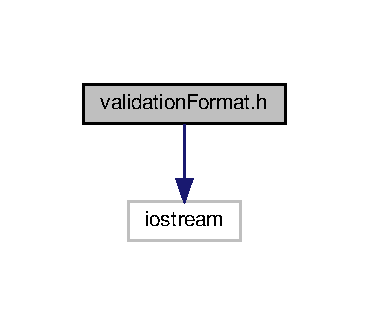
\includegraphics[width=177pt]{validationFormat_8h__incl}
\end{center}
\end{figure}
This graph shows which files directly or indirectly include this file\+:\nopagebreak
\begin{figure}[H]
\begin{center}
\leavevmode
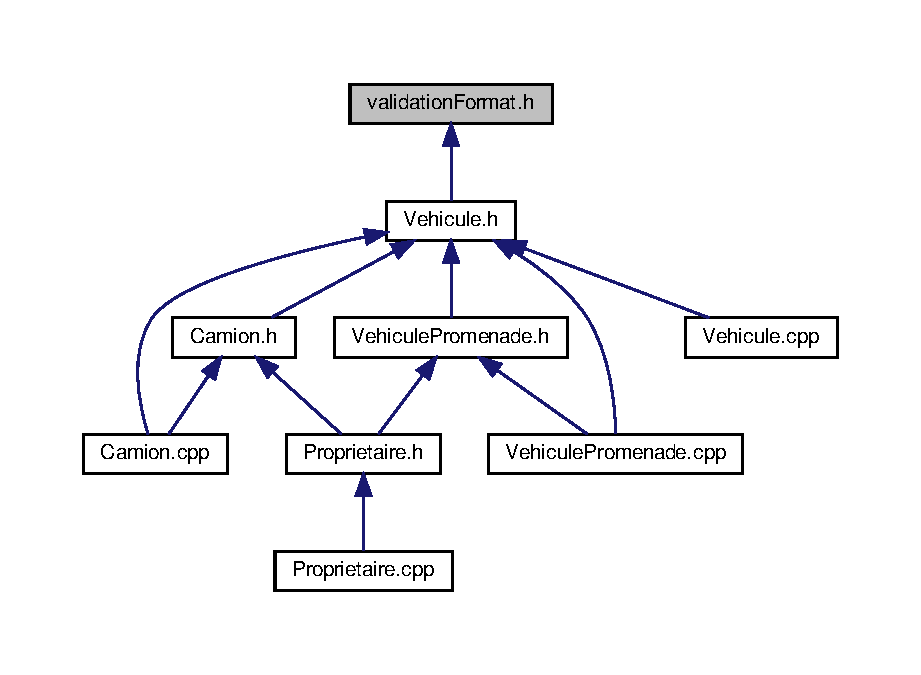
\includegraphics[width=350pt]{validationFormat_8h__dep__incl}
\end{center}
\end{figure}
\subsection*{Functions}
\begin{DoxyCompactItemize}
\item 
bool \hyperlink{validationFormat_8cpp_a54e96460aa1c34b195351e8bb3cffeef}{util\+::valider\+Immatriculation} (const std\+::string \&p\+\_\+immatriculation)
\begin{DoxyCompactList}\small\item\em Fonction qui permet de valider le format dune plaque dimmatriculation. \end{DoxyCompactList}\item 
bool \hyperlink{validationFormat_8cpp_a7bdc44b565fc0da4d7244670d00ce416}{util\+::valider\+Immatriculation\+Promenade} (const std\+::string \&p\+\_\+immatriculation)
\begin{DoxyCompactList}\small\item\em Fonction qui permet de valider le format dune plaque d\textquotesingle{}immatriculation de promenade. \end{DoxyCompactList}\item 
bool \hyperlink{validationFormat_8cpp_a4cf20d6bfbd40c3a521faafe28f1edde}{util\+::valider\+Immatriculation\+Camion} (const std\+::string \&p\+\_\+immatriculation)
\begin{DoxyCompactList}\small\item\em Fonction qui permet de valider le format dune plaque d\textquotesingle{}immatriculation de camion. \end{DoxyCompactList}\item 
bool \hyperlink{validationFormat_8cpp_a7d9e1cb34ea051b7bb3203e0045ae3a3}{util\+::valider\+Niv} (const std\+::string \&p\+\_\+niv)
\begin{DoxyCompactList}\small\item\em Fonction qui permet de valider le format dun N\+IV. \end{DoxyCompactList}\end{DoxyCompactItemize}


\subsection{Detailed Description}
Fichier permettant de valider une plaque automobile et un N\+IV. 

\begin{DoxyDate}{Date}
2019-\/10-\/15 
\end{DoxyDate}
\begin{DoxyAuthor}{Author}
Renaud Morin 
\end{DoxyAuthor}


\subsection{Function Documentation}
\mbox{\Hypertarget{validationFormat_8cpp_file_a54e96460aa1c34b195351e8bb3cffeef}\label{validationFormat_8cpp_file_a54e96460aa1c34b195351e8bb3cffeef}} 
\index{validation\+Format.\+h@{validation\+Format.\+h}!valider\+Immatriculation@{valider\+Immatriculation}}
\index{valider\+Immatriculation@{valider\+Immatriculation}!validation\+Format.\+h@{validation\+Format.\+h}}
\subsubsection{\texorpdfstring{valider\+Immatriculation()}{validerImmatriculation()}}
{\footnotesize\ttfamily bool util\+::valider\+Immatriculation (\begin{DoxyParamCaption}\item[{const std\+::string \&}]{p\+\_\+immatriculation }\end{DoxyParamCaption})}



Fonction qui permet de valider le format dune plaque dimmatriculation. 


\begin{DoxyParams}[1]{Parameters}
\mbox{\tt in}  & {\em p\+\_\+immatriculation} & numero de plaque a verifier \\
\hline
\end{DoxyParams}
\begin{DoxyReturn}{Returns}
valeur booléenne selon la validité de la plaque automobile 
\end{DoxyReturn}
\mbox{\Hypertarget{validationFormat_8cpp_file_a4cf20d6bfbd40c3a521faafe28f1edde}\label{validationFormat_8cpp_file_a4cf20d6bfbd40c3a521faafe28f1edde}} 
\index{validation\+Format.\+h@{validation\+Format.\+h}!valider\+Immatriculation\+Camion@{valider\+Immatriculation\+Camion}}
\index{valider\+Immatriculation\+Camion@{valider\+Immatriculation\+Camion}!validation\+Format.\+h@{validation\+Format.\+h}}
\subsubsection{\texorpdfstring{valider\+Immatriculation\+Camion()}{validerImmatriculationCamion()}}
{\footnotesize\ttfamily bool util\+::valider\+Immatriculation\+Camion (\begin{DoxyParamCaption}\item[{const std\+::string \&}]{p\+\_\+immatriculation }\end{DoxyParamCaption})}



Fonction qui permet de valider le format dune plaque d\textquotesingle{}immatriculation de camion. 


\begin{DoxyParams}[1]{Parameters}
\mbox{\tt in}  & {\em p\+\_\+immatriculation} & numero de plaque a verifier \\
\hline
\end{DoxyParams}
\begin{DoxyReturn}{Returns}
valeur booléenne selon la validité de la plaque de camion 
\end{DoxyReturn}
\mbox{\Hypertarget{validationFormat_8cpp_file_a7bdc44b565fc0da4d7244670d00ce416}\label{validationFormat_8cpp_file_a7bdc44b565fc0da4d7244670d00ce416}} 
\index{validation\+Format.\+h@{validation\+Format.\+h}!valider\+Immatriculation\+Promenade@{valider\+Immatriculation\+Promenade}}
\index{valider\+Immatriculation\+Promenade@{valider\+Immatriculation\+Promenade}!validation\+Format.\+h@{validation\+Format.\+h}}
\subsubsection{\texorpdfstring{valider\+Immatriculation\+Promenade()}{validerImmatriculationPromenade()}}
{\footnotesize\ttfamily bool util\+::valider\+Immatriculation\+Promenade (\begin{DoxyParamCaption}\item[{const std\+::string \&}]{p\+\_\+immatriculation }\end{DoxyParamCaption})}



Fonction qui permet de valider le format dune plaque d\textquotesingle{}immatriculation de promenade. 


\begin{DoxyParams}[1]{Parameters}
\mbox{\tt in}  & {\em p\+\_\+immatriculation} & numero de plaque a verifier \\
\hline
\end{DoxyParams}
\begin{DoxyReturn}{Returns}
valeur booléenne selon la validité de la plaque de vehicule de promenade 
\end{DoxyReturn}
\mbox{\Hypertarget{validationFormat_8cpp_file_a7d9e1cb34ea051b7bb3203e0045ae3a3}\label{validationFormat_8cpp_file_a7d9e1cb34ea051b7bb3203e0045ae3a3}} 
\index{validation\+Format.\+h@{validation\+Format.\+h}!valider\+Niv@{valider\+Niv}}
\index{valider\+Niv@{valider\+Niv}!validation\+Format.\+h@{validation\+Format.\+h}}
\subsubsection{\texorpdfstring{valider\+Niv()}{validerNiv()}}
{\footnotesize\ttfamily bool util\+::valider\+Niv (\begin{DoxyParamCaption}\item[{const std\+::string \&}]{p\+\_\+niv }\end{DoxyParamCaption})}



Fonction qui permet de valider le format dun N\+IV. 


\begin{DoxyParams}[1]{Parameters}
\mbox{\tt in}  & {\em p\+\_\+niv} & numero, N\+IV a verifier \\
\hline
\end{DoxyParams}
\begin{DoxyReturn}{Returns}
valeur booléenne selon la validité du N\+IV 
\end{DoxyReturn}

\hypertarget{Vehicule_8cpp}{}\section{Vehicule.\+cpp File Reference}
\label{Vehicule_8cpp}\index{Vehicule.\+cpp@{Vehicule.\+cpp}}


Fichier d\textquotesingle{}implémentation de la classe Vehicule.  


{\ttfamily \#include $<$iostream$>$}\newline
{\ttfamily \#include \char`\"{}Date.\+h\char`\"{}}\newline
{\ttfamily \#include \char`\"{}Vehicule.\+h\char`\"{}}\newline
{\ttfamily \#include $<$string$>$}\newline
{\ttfamily \#include $<$sstream$>$}\newline
Include dependency graph for Vehicule.\+cpp\+:\nopagebreak
\begin{figure}[H]
\begin{center}
\leavevmode
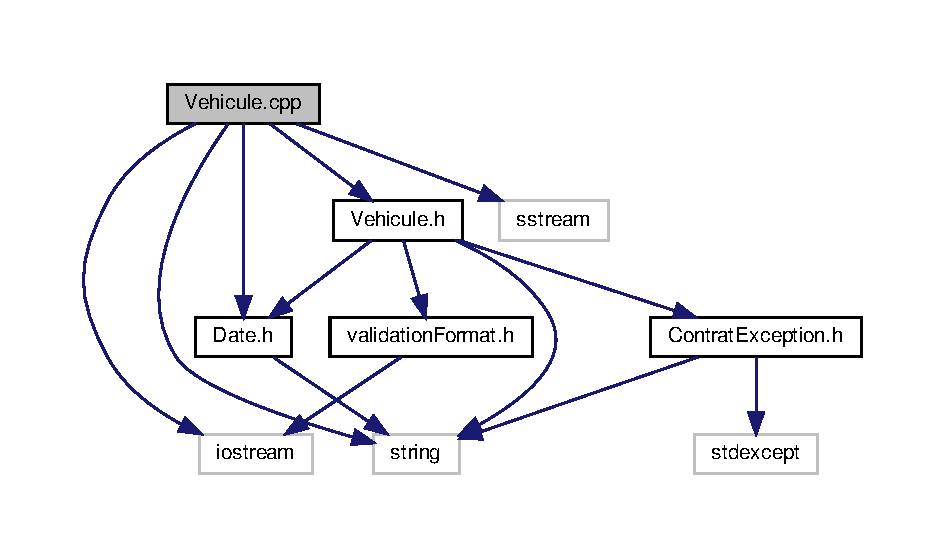
\includegraphics[width=350pt]{Vehicule_8cpp__incl}
\end{center}
\end{figure}


\subsection{Detailed Description}
Fichier d\textquotesingle{}implémentation de la classe Vehicule. 

\begin{DoxyDate}{Date}
2019-\/10-\/15 
\end{DoxyDate}
\begin{DoxyAuthor}{Author}
Renaud Morin 
\end{DoxyAuthor}

\hypertarget{Vehicule_8h}{}\section{Vehicule.\+h File Reference}
\label{Vehicule_8h}\index{Vehicule.\+h@{Vehicule.\+h}}


Fichier déclaration de la classe Vehicule.  


{\ttfamily \#include $<$string$>$}\newline
{\ttfamily \#include \char`\"{}Date.\+h\char`\"{}}\newline
{\ttfamily \#include \char`\"{}validation\+Format.\+h\char`\"{}}\newline
{\ttfamily \#include \char`\"{}Contrat\+Exception.\+h\char`\"{}}\newline
Include dependency graph for Vehicule.\+h\+:\nopagebreak
\begin{figure}[H]
\begin{center}
\leavevmode
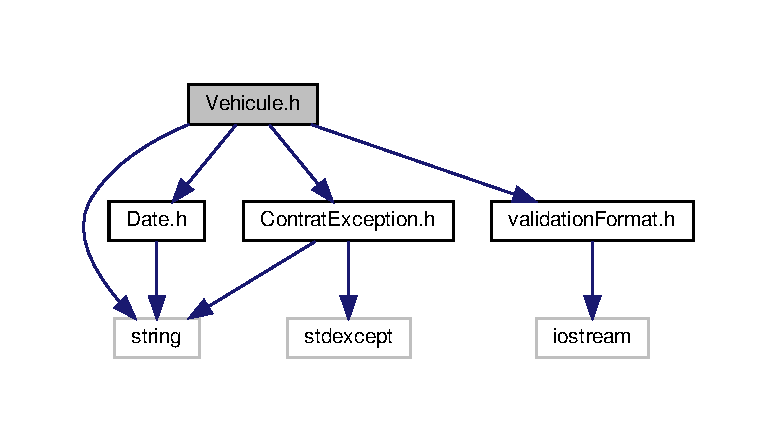
\includegraphics[width=350pt]{Vehicule_8h__incl}
\end{center}
\end{figure}
This graph shows which files directly or indirectly include this file\+:\nopagebreak
\begin{figure}[H]
\begin{center}
\leavevmode
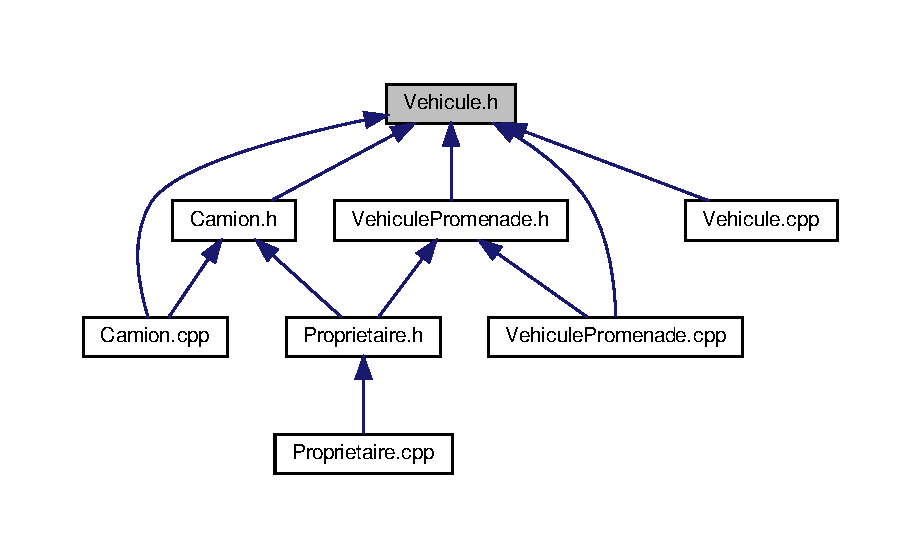
\includegraphics[width=350pt]{Vehicule_8h__dep__incl}
\end{center}
\end{figure}
\subsection*{Classes}
\begin{DoxyCompactItemize}
\item 
class \hyperlink{classsaaq_1_1Vehicule}{saaq\+::\+Vehicule}
\begin{DoxyCompactList}\small\item\em Classe vehicule qui contient les informations d\textquotesingle{}une plaque automobile. Contient la plaque d\textquotesingle{}immatriculation, la date d\textquotesingle{}enregistrement et le N\+IV du vehicule. Des méthode qui permettent de nous donner chaques valeurs. Une méthode qui permet d\textquotesingle{}assigner une nouvelle plaque de vehicule. Une méthode qui permet d\textquotesingle{}afficher le tout dans un format console. \end{DoxyCompactList}\end{DoxyCompactItemize}


\subsection{Detailed Description}
Fichier déclaration de la classe Vehicule. 

\begin{DoxyDate}{Date}
2019-\/10-\/15 
\end{DoxyDate}
\begin{DoxyAuthor}{Author}
Renaud Morin 
\end{DoxyAuthor}

\hypertarget{VehiculePromenade_8cpp}{}\section{Vehicule\+Promenade.\+cpp File Reference}
\label{VehiculePromenade_8cpp}\index{Vehicule\+Promenade.\+cpp@{Vehicule\+Promenade.\+cpp}}


Fichier d\textquotesingle{}implementation de la classe Vehicule\+Promenade.  


{\ttfamily \#include \char`\"{}Vehicule.\+h\char`\"{}}\newline
{\ttfamily \#include \char`\"{}Vehicule\+Promenade.\+h\char`\"{}}\newline
{\ttfamily \#include \char`\"{}Contrat\+Exception.\+h\char`\"{}}\newline
{\ttfamily \#include \char`\"{}Date.\+h\char`\"{}}\newline
{\ttfamily \#include $<$iostream$>$}\newline
{\ttfamily \#include $<$string$>$}\newline
{\ttfamily \#include $<$sstream$>$}\newline
Include dependency graph for Vehicule\+Promenade.\+cpp\+:\nopagebreak
\begin{figure}[H]
\begin{center}
\leavevmode
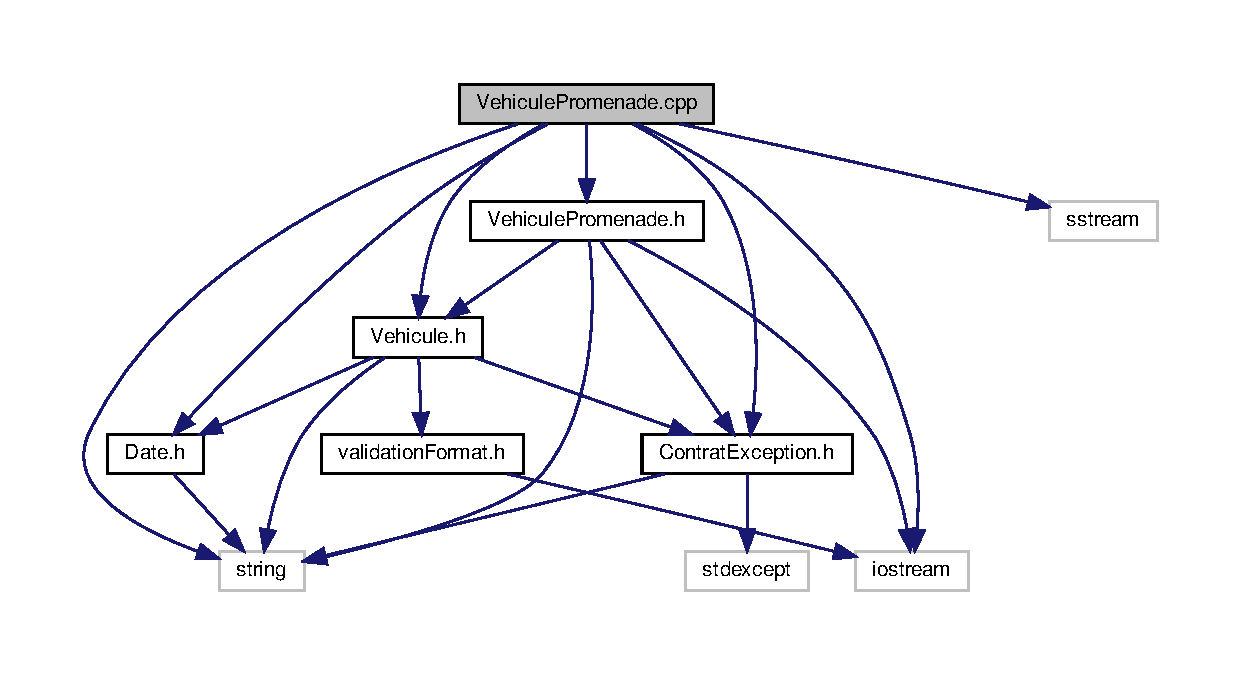
\includegraphics[width=350pt]{VehiculePromenade_8cpp__incl}
\end{center}
\end{figure}


\subsection{Detailed Description}
Fichier d\textquotesingle{}implementation de la classe Vehicule\+Promenade. 

\begin{DoxyDate}{Date}
2019-\/11-\/15 
\end{DoxyDate}
\begin{DoxyAuthor}{Author}
Renaud Morin 
\end{DoxyAuthor}

\hypertarget{VehiculePromenade_8h}{}\section{Vehicule\+Promenade.\+h File Reference}
\label{VehiculePromenade_8h}\index{Vehicule\+Promenade.\+h@{Vehicule\+Promenade.\+h}}


Fichier déclaration de la classe Vehicule\+Promenade.  


{\ttfamily \#include $<$iostream$>$}\newline
{\ttfamily \#include \char`\"{}Vehicule.\+h\char`\"{}}\newline
{\ttfamily \#include $<$string$>$}\newline
{\ttfamily \#include \char`\"{}Contrat\+Exception.\+h\char`\"{}}\newline
Include dependency graph for Vehicule\+Promenade.\+h\+:\nopagebreak
\begin{figure}[H]
\begin{center}
\leavevmode
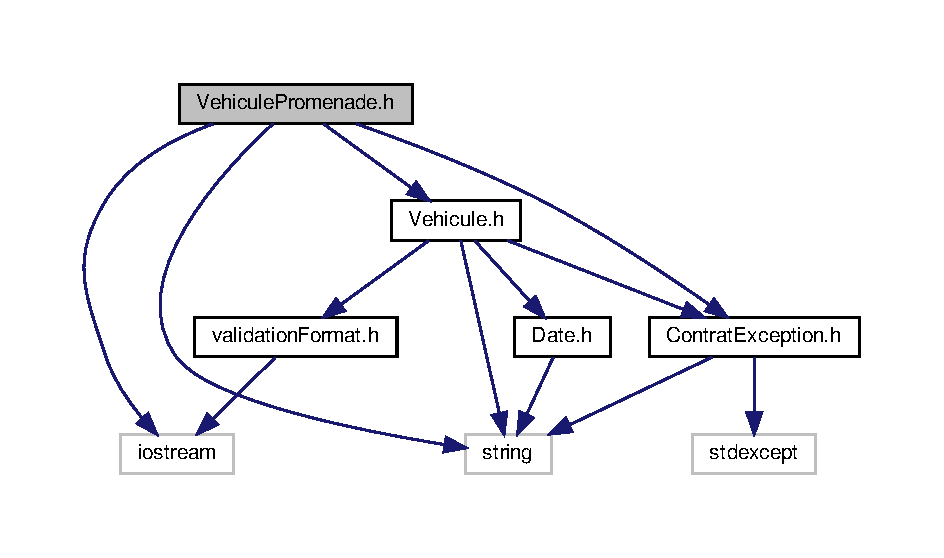
\includegraphics[width=350pt]{VehiculePromenade_8h__incl}
\end{center}
\end{figure}
This graph shows which files directly or indirectly include this file\+:\nopagebreak
\begin{figure}[H]
\begin{center}
\leavevmode
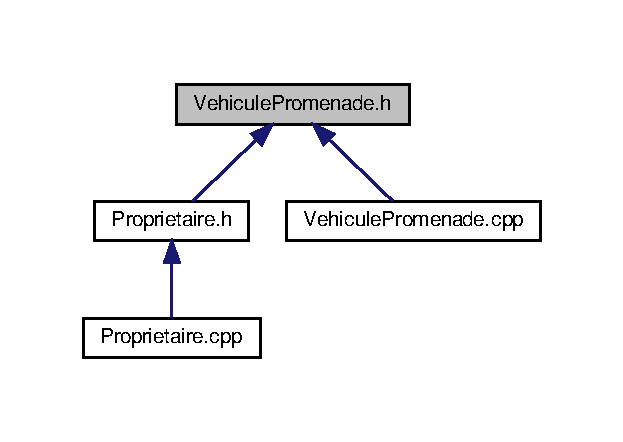
\includegraphics[width=299pt]{VehiculePromenade_8h__dep__incl}
\end{center}
\end{figure}
\subsection*{Classes}
\begin{DoxyCompactItemize}
\item 
class \hyperlink{classsaaq_1_1VehiculePromenade}{saaq\+::\+Vehicule\+Promenade}
\begin{DoxyCompactList}\small\item\em Classe \hyperlink{classsaaq_1_1VehiculePromenade}{Vehicule\+Promenade} qui contient les informations sur un \hyperlink{classsaaq_1_1Vehicule}{Vehicule} de Promenade Contient la plaque d\textquotesingle{}immatriculation, la date d\textquotesingle{}enregistrement, le nombre de place et le N\+IV du vehicule. Des méthode qui permettent de nous donner chaques valeurs. Une méthode qui permet d\textquotesingle{}assigner une nouvelle plaque de \hyperlink{classsaaq_1_1Vehicule}{Vehicule} de Promenade. Une méthode qui permet d\textquotesingle{}afficher le tout dans un format console. \end{DoxyCompactList}\end{DoxyCompactItemize}


\subsection{Detailed Description}
Fichier déclaration de la classe Vehicule\+Promenade. 

\begin{DoxyDate}{Date}
2019-\/11-\/15 
\end{DoxyDate}
\begin{DoxyAuthor}{Author}
Renaud Morin 
\end{DoxyAuthor}

%--- End generated contents ---

% Index
\backmatter
\newpage
\phantomsection
\clearemptydoublepage
\addcontentsline{toc}{chapter}{Index}
\printindex

\end{document}
